%%%%%%%%%%%%%%%%%%%%%%%%%%%%%%%%%%%%%%%%%%%%%%%%%%%%%%%%%%%%%%%%%%
%%%%%%%%%%%%%%%%%%%%%%%%%%%%%%%%%%%%%%%%%%%%%%%%%%%%%%%%%%%%%%%%%%
\chapter{Erste Schritte}
\label{sec:firstSteps}
%%%%%%%%%%%%%%%%%%%%%%%%%%%%%%%%%%%%%%%%%%%%%%%%%%%%%%%%%%%%%%%%%%
%%%%%%%%%%%%%%%%%%%%%%%%%%%%%%%%%%%%%%%%%%%%%%%%%%%%%%%%%%%%%%%%%%

%%%%%%%%%%%%%%%%%%%%%%%%%%%%%%%%%%%%%%%%%%%%%%%%%%%%%%%%%%%%%%%%%%
%%%%%%%%%%%%%%%%%%%%%%%%%%%%%%%%%%%%%%%%%%%%%%%%%%%%%%%%%%%%%%%%%%
\section{Vorstellung}
\label{sec:intro}
%%%%%%%%%%%%%%%%%%%%%%%%%%%%%%%%%%%%%%%%%%%%%%%%%%%%%%%%%%%%%%%%%%
%%%%%%%%%%%%%%%%%%%%%%%%%%%%%%%%%%%%%%%%%%%%%%%%%%%%%%%%%%%%%%%%%%

R ist eine freie und kostenlose Software-Umgebung zur statistischen Datenanalyse \cite{Ihaka1996, RDevelopmentCoreTeam2008c}. R integriert eine Vielzahl von Möglichkeiten, um Daten organisieren, transformieren, auswerten und visualisieren zu können. Dabei bezeichnet R sowohl das Programm selbst als auch die Sprache, in der die Auswertungsbefehle geschrieben werden.\footnote{Genauer gesagt ist GNU R ursprünglich eine \emph{open source} Implementierung der Sprache\index{S} S \cite{Becker1988}. Der open source Programmen zugrundeliegende Quelltext ist frei erhältlich, zudem darf die Software frei genutzt, verbreitet und verändert werden. Genaueres erläutert der Befehl \lstinline!licence()!. Kommerzielle Varianten von R sind u.\,a.\ Microsoft R \cite{Revolution2014} und TIBCO TERR \cite{TIBCOSoftwareInc2008}.} Denn in R bestehen Auswertungen aus einer Abfolge von Befehlen in Textform, die unter Einhaltung einer bestimmten Syntax selbst einzugeben sind. Jeder Befehl stellt dabei einen eigenen Auswertungsschritt dar, wobei eine vollständige Datenanalyse die Abfolge vieler solcher Schritte umfasst. So könnte man Daten zunächst aus einer Datei lesen, sie dann prüfen und geeignet transformieren, um dann eine Teilmenge von Beobachtungen auszuwählen und mit ihr einen statistischen Test durchzuführen, dessen Ergebnisse im Anschluss in einem Diagramm visualisiert werden.

%%%%%%%%%%%%%%%%%%%%%%%%%%%%%%%%%%%%%%%%%%%%%%%%%%%%%%%%%%%%%%%%%%
%%%%%%%%%%%%%%%%%%%%%%%%%%%%%%%%%%%%%%%%%%%%%%%%%%%%%%%%%%%%%%%%%%
\subsection{Pro und Contra R}
%%%%%%%%%%%%%%%%%%%%%%%%%%%%%%%%%%%%%%%%%%%%%%%%%%%%%%%%%%%%%%%%%%
%%%%%%%%%%%%%%%%%%%%%%%%%%%%%%%%%%%%%%%%%%%%%%%%%%%%%%%%%%%%%%%%%%

Während in Programmen, die über eine grafische Benutzeroberfläche gesteuert werden, die Auswahl von vorgegebenen Menüpunkten einen wesentlichen Teil der Arbeit ausmacht, ist es in R die aktive Produktion von Befehlsausdrücken. Diese Eigenschaft ist gleichzeitig ein wesentlicher Vorteil wie auch eine Herausforderung beim Einstieg in die Arbeit mit R. Zu den Vorteilen von R zählen:

\begin{itemize}
\item Die befehlsgesteuerte Arbeitsweise stellt sicher, dasss einmal erstellte Auswertungen später leicht angepasst und erweitert werden können. Sie erhöht durch die Wiederverwendbarkeit von bewährten Befehlssequenzen für typische Arbeitsschritte auch langfristig die Effizienz und Zuverlässigkeit von Analysen.
\item Die Möglichkeit zur Weitergabe von Befehlssequenzen mit den zugehörigen Datensätzen an Dritte kann die Auswertung für andere transparent und überprüfbar machen. Auf diese Weise lassen sich Auswertungen selbst und durch andere genau reproduzieren, wodurch die Auswertungsobjektivität steigt.
\item R-Auswertungen lassen sich in Dokumente einbetten, die beschreibenden Text, R-Befehle und die automatisch erzeugte Ausgabe dieser Befehle enthalten -- inkl.\ Diagramme und Tabellen (Abschn.\ \ref{sec:rmd}). Auswertungen lassen sich sogar als interaktive Web-Anwendungen veröffentlichen. Indem Hintergrundinformationen, Details zur Auswertung sowie Ergebnisse kombiniert werden, bietet R eine umfassende Plattform für transparente, reproduzierbare statistische Analysen (Abschn.\ \ref{sec:reproducibility}).
\item R ist kostenlos und sowohl für Windows als auch für MacOS und Linux frei verfügbar. R kann dadurch ohne Einschränkungen in jedem Kontext -- beruflich, privat, in der Ausbildung -- und unabhängig von den finanziellen Möglichkeiten von allen verwendet werden.
\item Als freies open source Programm wird R beständig von vielen Personen evaluiert, weiterentwickelt und verbessert (vgl.\ \citeNP{RFoundation2013} für eingesetzte Methoden der Qualitätssicherung). Da der Quelltext frei verfügbar ist und zudem viele Auswertungsfunktionen ihrerseits in R geschrieben sind, ist die Art der Berechnung statistischer Kennwerte vollständig transparent. Sie kann damit bei Interesse analysiert und auf Richtigkeit kontrolliert werden.
\item Dank seines modularen Aufbaus bietet R die Möglichkeit, die Basisfunktionalität für spezielle Anwendungszwecke durch eigenständig entwickelte Zusatzkomponenten (\emph{Pakete}) zu erweitern, von denen bereits viele tausend frei verfügbar sind (Abschn.\ \ref{sec:packages}).
\item Auch ohne tiefergehende Programmierkenntnisse lassen sich in R eigene Funktionen erstellen und so Auswertungen flexibel an individuelle Anforderungen anpassen. Da Funktionen in derselben Syntax wie normale Auswertungen geschrieben werden, sind dafür zunächst nur wenige Zusatzschritte zu erlernen (Kap.\ \ref{sec:programming}). Reine Anwender können sich schrittweise zu R Entwicklern weiterentwickeln, wobei R angepasst an die individuellen Anforderungen {\quotedblbase}mitwächst{\textquotedblleft}.
\item In den vergangenen Jahren hat sich eine sehr lebhafte, inhaltlich vielseitige und hilfsbereite Online-Community um R entwickelt, die in Email-Verteilern, Blogs, Online-Kursen und Video-Tutorials viel Unterstützung liefert (Abschn.\ \ref{sec:documentation}).
\end{itemize}

R hält für Anwender allerdings auch Hürden bereit, insbesondere für Einsteiger, die nur Erfahrung mit Programmen besitzen, die über eine grafische Benutzeroberfläche bedient werden \cite{Muenchen2018}:
\begin{itemize}
\item Die einzelnen Befehle und ihre Syntax zu erlernen, erfordert die Bereitschaft zur Einübung. Es muss zunächst ein Grundverständnis für die Arbeitsabläufe sowie ein gewisser {\quotedblbase}Wortschatz{\textquotedblleft} häufiger Funktionen und Konzepte geschaffen werden, ehe Daten umfassend ausgewertet werden können.
\item Im Gegensatz zu Programmen mit grafischer Benutzeroberfläche müssen Befehle aktiv erinnert werden. Es stehen keine Gedächtnisstützen i.\,S.\ von Elementen einer grafischen Umgebung zur Verfügung, die interaktiv mögliche Vorgehensweisen anbieten und zu einem Wiedererkennen führen könnten. Dies betrifft sowohl die Auswahl von geeigneten Analysen als auch die konkrete Umsetzung von Arbeitsschritten.
\item Anders als in kommerzieller Statistik-Software gibt es in R keine festgelegte, standardisierte Vorgehensweise für einen bestimmten Auswertungsschritt. Stattdessen führen meist mehrere Ansätze zum selben Ergebnis. Dies gilt insbesondere durch die Funktionalität von Zusatzpaketen, die sich untereinander, aber auch mit dem Basisumfang von R überschneiden kann. Deshalb machen auch Bücher oder Online-Tutorials oft uneinheitliche Empfehlungen. Diese Flexibilität und Vielfalt kann zu Beginn für Verwirrung und Unsicherheit sorgen, welcher Weg zum Ziel am besten gewählt werden sollte.
\item Während natürliche Sprache sehr fehlertolerant ist, müssen Befehle in R immer exakt richtig eingegeben werden. Dies kann zu Beginn frustrierend und auch zeitraubend sein, weil schon vermeintlich unwesentliche Fehler verhindern, dass Befehle ausgeführt werden (Abschn.\ \ref{sec:mistakes}). Im Fall falsch eingegebener Befehle liefert R aber Fehlermeldungen, die Rückschlüsse auf die Ursache erlauben. Moderne Entwicklungsumgebungen helfen durch visuelle Hinweise dabei, Syntaxfehler zu vermeiden (Abschn.\ \ref{sec:gui}).
\item Bei der Analyse extrem großer Datenmengen besteht gegenwärtig das Problem, dass R Datensätze zur Bearbeitung im Arbeitsspeicher vorhalten muss, was die Größe von praktisch auswertbaren Datensätzen einschränkt. Hinweise zu Lösungsansätzen sowie zur Ausnutzung paralleler Rechnerarchitekturen finden sich in Abschn.\ \ref{sec:performance}.
\end{itemize}

Startschwierigkeiten sind beim Lernen von R zu erwarten, sollten jedoch niemanden entmutigen: Auch wenn dies zu Beginn häufige Fehler mit sich bringt, ist vielmehr ein spielerisch-exploratives Kennenlernen wichtig, um ein besseres Verständnis der Grundprinzipien zu entwickeln. Ein wichtiger Grundsatz ist dabei, sich zunächst inhaltlich zu überlegen, welche Teilschritte für eine konkrete Auswertung notwendig sind. Je konkreter die Teilschritte dieses gedanklichen Ablaufplans sind, desto einfacher lassen sich ihnen einzelne Befehlsbausteine zuordnen. Sind dann aus einfachen Auswertungen viele solcher Befehlsbausteine vertraut, lassen sie sich Schritt für Schritt zu komplexen Analysen zusammenstellen.

%%%%%%%%%%%%%%%%%%%%%%%%%%%%%%%%%%%%%%%%%%%%%%%%%%%%%%%%%%%%%%%%%%
%%%%%%%%%%%%%%%%%%%%%%%%%%%%%%%%%%%%%%%%%%%%%%%%%%%%%%%%%%%%%%%%%%
\subsection{Typografische Konventionen}
%%%%%%%%%%%%%%%%%%%%%%%%%%%%%%%%%%%%%%%%%%%%%%%%%%%%%%%%%%%%%%%%%%
%%%%%%%%%%%%%%%%%%%%%%%%%%%%%%%%%%%%%%%%%%%%%%%%%%%%%%%%%%%%%%%%%%

\index{Notation}
Zur besseren Lesbarkeit sollen zunächst einige typografische Konventionen für die Notation vereinbart werden. Um zwischen den Befehlen und Ausgaben von R sowie der zugehörigen Beschreibung innerhalb dieses Textes unterscheiden zu können, werden Befehle und Ausgaben im Schrifttyp \myURL{Schreibmaschine} dargestellt. Eine Befehlszeile mit zugehöriger Ausgabe könnte also z.\,B.\ so aussehen:
\begin{lstlisting}
> 1 + 1
[1] 2
\end{lstlisting}

Die erste Zeile bezeichnet dabei die Eingabe des Anwenders, die zweite Zeile die (in diesem Text bisweilen leicht umformatierte) Ausgabe von R. Fehlen Teile der Ausgabe im Text, ist dies mit \lstinline!...! als Auslassungszeichen angedeutet. Zeilenumbrüche innerhalb von R-Befehlen sind durch Pfeile in der Form \lstinline!Befehl Anfang! {\tiny$\searrow \quad \rightarrow$} \lstinline!Fortsetzung! gekennzeichnet, um deutlich zu machen, dass die getrennten Teile unmittelbar zusammen gehören. Platzhalter, wie z.\,B.\ \lstinline[language=]!<<Dateiname>>!, die für einen Typ von Objekten stehen (hier Dateien) und mit einem beliebigen konkreten Objekt dieses Typs gefüllt werden können, werden in stumpfwinklige Klammern \lstinline!<<>>! gesetzt.

Internet-URLs, Tastenkombinationen sowie Dateien und Verzeichnisse werden im Schrifttyp \myURL{Schreibmaschine} dargestellt, wobei die Unterscheidung zu R-Befehlen aus dem Kontext hervorgeht.

%%%%%%%%%%%%%%%%%%%%%%%%%%%%%%%%%%%%%%%%%%%%%%%%%%%%%%%%%%%%%%%%%%
%%%%%%%%%%%%%%%%%%%%%%%%%%%%%%%%%%%%%%%%%%%%%%%%%%%%%%%%%%%%%%%%%%
\subsection{R installieren}
%%%%%%%%%%%%%%%%%%%%%%%%%%%%%%%%%%%%%%%%%%%%%%%%%%%%%%%%%%%%%%%%%%
%%%%%%%%%%%%%%%%%%%%%%%%%%%%%%%%%%%%%%%%%%%%%%%%%%%%%%%%%%%%%%%%%%

\index{Installation}
\index{download}
\index{herunterladen|see{download}}
\index{Homepage}
Die Homepage des R-Projekts ist die zentrale Anlaufstelle für Nachrichten über die Entwicklung von R, für den \emph{download} des Programms selbst, für Zusatzpakete sowie für frei verfügbare Literatur:

\url{https://www.r-project.org/}

Die folgenden Ausführungen beziehen sich auf die Installation des R-Basispakets unter Windows $10$, vgl.\ dazu auch die offizielle Installationsanleitung \cite{RDevelopmentCoreTeam2008a} und die Windows-FAQ \cite{Ripley2008}.\footnote{Abgesehen von der Oberfläche und abweichenden Pfadangaben bestehen nur unwesentliche Unterschiede zwischen der Arbeit mit R unter verschiedenen Betriebssystemen.} Für die Installationsdatei des Programms folgt man auf der Projektseite dem Verweis \myURL{Download, Packages / CRAN}, der auf eine Übersicht von CRAN-servern verweist, von denen die Dateien erhältlich sind.\footnote{CRAN (\emph{Comprehensive R Archive Network}) bezeichnet ein weltweites Netzwerk von \emph{mirror servern} für R-Installationsdateien, Zusatzpakete und offizielle Dokumentation. Eine durchsuchbare und übersichtlichere Oberfläche mit weiteren Funktionen ist \url{https://r-pkg.org/}.} Nach der Wahl eines CRAN-servers gelangt man über \myURL{Download and Install R / Download R for Windows: base} zum Verzeichnis mit der Installationsdatei \myURL{R-4.0.0-win.exe}, die auf dem eigenen Rechner zu speichern ist.\footnote{R Version 4.0.0 wird im Frühjahr 2020 veröffentlicht. Neuere Versionen erscheinen ca.\ halbjährlich. Dabei sind leichte, für den Benutzer jedoch üblicherweise nicht merkliche Abweichungen zur in diesem Manuskript beschriebenen Arbeitsweise von Funktionen möglich.}

Um R zu installieren, ist die gespeicherte Installationsdatei \lstinline[language=]!R-<<Version>>-win.exe! auszuführen und den Aufforderungen des Setup-Assistenten zu folgen. Die Installation setzt voraus, dass der Benutzer ausreichende Schreibrechte auf dem Computer besitzt, weshalb es u.\,U.\ notwendig ist, R als Administrator zu installieren. Wenn keine Änderungen am Installationsordner von R vorgenommen wurden, sollte R daraufhin im Verzeichnis \lstinline[language=]!C:\Programme\R-<<Version>>\! installiert sein, was sich in R mit\index[func]{Sys.getenv()@\lstinline{Sys.getenv()}} \lstinline!Sys.getenv("R_HOME")! prüfen lässt.

Unter MacOS verläuft die Installation analog, wobei den entsprechenden CRAN-links zur Installationsdatei zu folgen ist. Für einige Funktionen muss X11-Unterstützung über die XQuartz-Software zusätzlich installiert werden\footnote{\url{https://www.xquartz.org/}}. R ist in allen gängigen Linux-Distributionen enthalten und kann dort am einfachsten direkt über den jeweils verwendeten Paketmanager installiert werden. Unter Ubuntu und darauf aufbauenden Distributionen heißt das Basispaket \lstinline!r-base!, unter SUSE \lstinline!R-base! und unter RedHat/Fedora \lstinline!R!.

Eine vollständige virtualisierte R Umgebung bietet das \emph{Rocker} Projekt für die Container-Software Docker \cite{Boettiger2017}.\footnote{\url{https://www.rocker-project.org/}} Auf diesem Weg kann R auch online auf einer Cloud-Plattform gehostet werden.

%%%%%%%%%%%%%%%%%%%%%%%%%%%%%%%%%%%%%%%%%%%%%%%%%%%%%%%%%%%%%%%%%%
%%%%%%%%%%%%%%%%%%%%%%%%%%%%%%%%%%%%%%%%%%%%%%%%%%%%%%%%%%%%%%%%%%
\subsection{Grafische Benutzeroberflächen}
\label{sec:gui}
%%%%%%%%%%%%%%%%%%%%%%%%%%%%%%%%%%%%%%%%%%%%%%%%%%%%%%%%%%%%%%%%%%
%%%%%%%%%%%%%%%%%%%%%%%%%%%%%%%%%%%%%%%%%%%%%%%%%%%%%%%%%%%%%%%%%%

\index{grafische Benutzeroberflache@grafische Benutzeroberfläche}
\index{GUI|see{grafische Benutzeroberfläche}}
\index{Editor}
Obwohl es nicht zwingend notwendig ist, sollte zusätzlich zur Basis-Oberfläche von R eine komfortablere grafische Umgebung zur Befehlseingabe installiert werden. Eine solche alternative grafische Umgebung setzt dabei voraus, dass R selbst bereits installiert wurde.

\begin{itemize}
\item Die\index{RStudio@RStudio} auf R zugeschnittene Entwicklungsumgebung RStudio \cite{Allaire2011} ist frei verfügbar, einfach zu installieren, läuft unter mehreren Betriebssystemen mit einer konsistenten Oberfläche und erleichtert häufige Arbeitsschritte (Abschn.\ \ref{sec:console}). Zudem unterstützt RStudio besonders gut die Möglichkeiten, Dokumente mit eingebetteten R-Auswertungen zu erstellen (Abschn.\ \ref{sec:rmd}).
\item Eclipse StatET \cite{Wahlbrink2008} ist eine auf R zugeschnittene Variante der freien Entwicklungsumgebung Eclipse, die besonders für die Programmiersprache Java populär ist. Analog existiert auch für die auf Python spezialisierte Entwicklungsumgebung PyCharm ein Plugin zur Arbeit mit R \cite{JetBrains2020}.
\item Die freie Entwicklungsumgebung JupyterLab \cite{Kluyver2016} wurde ursprünglich für \emph{data science}-orientierte Anwendungen der Programmiersprache Python erstellt, kann aber ebenfalls mit R verwendet werden. Die Installation erfolgt am einfachsten über die Anaconda Distribution\footnote{\url{https://www.anaconda.com/}} und die separat zu installierende Software IRKernel.\footnote{\url{https://irkernel.github.io/}}
\item Der freie und plattformunabhängige Texteditor Emacs lässt sich ebenso wie XEmacs mit dem Zusatzpaket ESS (\emph{Emacs Speaks Statistics}, \citeNP{Rossini2014}) zu einer textbasierten Entwicklungsumgebung für R erweitern. Zielgruppe sind vor allem fortgeschrittene Anwender, die bereits mit Emacs vertraut sind.
%\item Unter Windows eignet sich etwa Tinn-R \cite{Faria2010}, um lediglich den R-eigenen Texteditor zu ersetzen.
%\item Das Zusatzpaket \index[pack]{JGR@\lstinline{JGR}} \lstinline!JGR! (\citeNP{Helbig2005}, Abschn.\ \ref{sec:packages}) stellt eine plattformunabhängige Oberfläche bereit, die der R-eigenen Oberfläche unter Windows sehr ähnlich ist.
\item Schließlich existieren Programme, die Analysefunktionen über grafische Menüs und damit ohne Befehlseingabe nutzbar machen, darunter Rcmdr \cite{Fox2017} und RKWard \cite{Roediger2012}. Diese Programme bieten derzeit jedoch nur Zugang zu einem Teil der Möglichkeiten von R.
\end{itemize}

%%%%%%%%%%%%%%%%%%%%%%%%%%%%%%%%%%%%%%%%%%%%%%%%%%%%%%%%%%%%%%%%%%
%%%%%%%%%%%%%%%%%%%%%%%%%%%%%%%%%%%%%%%%%%%%%%%%%%%%%%%%%%%%%%%%%%
\subsection{Weiterführende Informationsquellen und Literatur}
\label{sec:documentation}
%%%%%%%%%%%%%%%%%%%%%%%%%%%%%%%%%%%%%%%%%%%%%%%%%%%%%%%%%%%%%%%%%%
%%%%%%%%%%%%%%%%%%%%%%%%%%%%%%%%%%%%%%%%%%%%%%%%%%%%%%%%%%%%%%%%%%

\index{Literatur}
\index{Dokumentation|see{Literatur}}
\index{download}
\index{herunterladen|see{download}}
\index{Homepage}
\index{Hilfe!Internet}
Häufige Fragen zu R sowie speziell zur Verwendung von R unter Windows werden in den FAQ (\emph{frequently asked questions})\index{FAQ} beantwortet \cite{Hornik2009, Ripley2008}. Für individuelle Fragen existiert die Mailing-Liste\index{Mailing-Liste} \emph{R-help}, deren Adresse auf der Projektseite unter \myURL{R Project / Mailing Lists} genannt wird. Bevor sie für eigene Hilfegesuche genutzt wird, sollte eine selbständige Recherche vorausgehen. Zudem sind die Hinweise des \emph{posting-guide}\footnote{\url{https://www.r-project.org/posting-guide.html}} zu beherzigen, wobei ein einfaches reproduzierbares Beispiel besonders wichtig ist (Abschn.\ \ref{sec:reproducibility}).\footnote{\url{https://stackoverflow.com/q/5963269}} Beides gilt auch für das hilfreiche Web-Forum StackOverflow.\footnote{%
\url{https://stackoverflow.com/tags/R} -- \url{https://stats.stackexchange.com/tags/R}}
Kostenlose Online-Kurse werden etwa von edX angeboten.\footnote{%
%\url{https://www.datacamp.com/courses/free-introduction-to-r}\\
%\url{https://www.coursera.org/specializations/jhu-data-science}\\
\url{https://www.edx.org/course/statistics-and-r}\\
\url{https://www.edx.org/course/introduction-to-r-for-data-science-2}} Der Twitter \emph{hashtag} lautet \myURL{\#rstats}.

% Die Suche innerhalb von Beiträgen auf der Mailing-Liste, sowie innerhalb von Funktionen und der Hilfe erleichtert die auf R-Inhalte spezialisierte Seite Rdocumentation.\footnote{\url{http://www.rdocumentation.org/}}

Unter dem link \myURL{Documentation / Manuals} auf der Projektseite von R findet sich die vom R Entwickler-Team herausgegebene offizielle Dokumentation. Sie liefert einerseits einen umfassenden, aber sehr konzisen Überblick über R selbst \cite{Venables2008} und befasst sich andererseits mit Spezialthemen wie dem Datenaustausch mit anderen Programmen (Abschn.\ \ref{sec:dataImport}).% Weitere, von Anwendern beigesteuerte Literatur zu R findet sich auf der Projektseite unter dem Verweis \myURL{Documentation / Other}.
Darüber hinaus existiert eine Reihe von Büchern mit unterschiedlicher inhaltlicher Ausrichtung, die R-Projektseite bietet dazu unter \myURL{Documentation / Books} eine laufend aktualisierte Literaturübersicht:

\index{Hilfe!Literatur}
\index{Zeitreihen}
\index{räumliche Statistik}
\index{Karten|see{räumliche Statistik}}
\begin{itemize}
\item Eine empfehlenswerte Einführung in R anhand grundlegender statistischer Themen findet man etwa bei \citeA{Maindonald2007}. \citeA{Everitt2006} sowie \citeA{Venables2002} behandeln den Einsatz von R für fortgeschrittene statistische Anwendungen.
\item Für die Umsetzung spezieller statistischer Themen existieren eigene Bücher -- etwa zu
\begin{itemize}
\item Regressionsmodellen \cite{Fox2002,HarrellJr2001}
\item multivariaten Verfahren \cite{Zelterman2015}
\item gemischten linearen Modellen \cite{Galecki2013,Pinheiro2000,West2006}
\item Resampling-Verfahren \cite{Chernik2011,Chihara2011}
\item Zeitreihen \cite{Shumway2006,Hyndman2019}
\item Bayes-Methoden \cite{Kruschke2015,McElreath2015}
\item räumlicher Statistik \cite{Bivand2013}.
\end{itemize}
\item \citeA{Muenchen2008,Muenchen2010} sowie \citeA{Kleinman2014} richten sich speziell an Umsteiger von anderen Statistikpaketen wie SPSS, SAS oder Stata.
\item Einen Fokus auf R im Umfeld von data science und Maschinen-Lernen legen \citeA{Hastie2009,James2013b} sowie \citeA{Wickham2016a}.
\item Das Gebiet der Programmierung mit R wird von \citeA{Chambers2008, Gillespie2017} sowie \citeA{Wickham2014a} thematisiert.
\item \citeA{Murrell2005, Chang2013} und \citeA{Unwin2015} erläutern detailliert, wie Diagramme mit R erstellt werden können.
\item \citeA{Xie2013} sowie \citeA{Xie2018} behandeln, wie sich mit R dynamische Dokumente erstellen lassen, die Berechnungen, Ergebnisse und Beschreibungen integrieren.
\item Wie interaktive Web-Anwendungen mit dem Paket \lstinline!shiny!\index[pack]{shiny@\lstinline{shiny}} \cite{RStudioShiny2014} entwickelt werden können, zeigen \citeA{Sievert2020} und \citeA{Wickham2020}.
\end{itemize}

%%%%%%%%%%%%%%%%%%%%%%%%%%%%%%%%%%%%%%%%%%%%%%%%%%%%%%%%%%%%%%%%%%
%%%%%%%%%%%%%%%%%%%%%%%%%%%%%%%%%%%%%%%%%%%%%%%%%%%%%%%%%%%%%%%%%%
\section{Grundlegende Elemente}
%%%%%%%%%%%%%%%%%%%%%%%%%%%%%%%%%%%%%%%%%%%%%%%%%%%%%%%%%%%%%%%%%%
%%%%%%%%%%%%%%%%%%%%%%%%%%%%%%%%%%%%%%%%%%%%%%%%%%%%%%%%%%%%%%%%%%

%%%%%%%%%%%%%%%%%%%%%%%%%%%%%%%%%%%%%%%%%%%%%%%%%%%%%%%%%%%%%%%%%%
%%%%%%%%%%%%%%%%%%%%%%%%%%%%%%%%%%%%%%%%%%%%%%%%%%%%%%%%%%%%%%%%%%
\subsection{R Starten, beenden und die Konsole verwenden}
\label{sec:console}
%%%%%%%%%%%%%%%%%%%%%%%%%%%%%%%%%%%%%%%%%%%%%%%%%%%%%%%%%%%%%%%%%%
%%%%%%%%%%%%%%%%%%%%%%%%%%%%%%%%%%%%%%%%%%%%%%%%%%%%%%%%%%%%%%%%%%

\index{starten}
Nach der Installation lässt sich R unter Windows über die bei der Installation erstellte Verknüpfung auf dem desktop bzw.\ im Startmenü starten. Hierdurch öffnen sich zwei Fenster: ein großes, das Programmfenster, und darin ein kleineres, die\index{Konsole} \emph{Konsole}. Unter MacOS und Linux ist die Konsole das einzige sich öffnende Fenster.

\index{RStudio@RStudio}
Der Arbeitsbereich der Entwicklungsumgebung RStudio gliedert sich in vier Regionen (Abb.\ \ref{fig:rstudio}):\footnote{RStudio wird derzeit mit hohem Tempo weiterentwickelt. Es ist deshalb möglich, dass im Laufe der Zeit Aussehen und Funktionalität in Details von der folgenden Beschreibung abweichen.}

\begin{itemize}
\item Links unten befindet sich die Konsole zur interaktiven Arbeit mit R. Befehle können direkt auf der Konsole eingegeben werden, außerdem erscheint die Ausgabe von R hier.
\item Links oben öffnet sich ein Editor, in dem über das Menü \emph{File} \textrightarrow\ \emph{New File} \textrightarrow\ \emph{R Script} ein eigenes Befehlsskript erstellt oder über \emph{File} \textrightarrow\ \emph{Open File} ein bereits vorhandenes Befehlsskript geöffnet werden kann. Ein Skript ist dabei eine einfache Textdatei mit einer Sammlung von nacheinander abzuarbeitenden Befehlen (Abschn.\ \ref{sec:scripting}). Die Befehle eines Skripts können im Editor markiert und mit dem icon \emph{Run} bzw.\ mit der Tastenkombination \myURL{Strg+Return} (unter MacOS \texttt{Cmd+Return}) an die Konsole gesendet werden.
\item Rechts oben befinden sich zwei Tabs: \emph{Environment} zeigt alle derzeit verfügbaren Objekte an -- etwa Datensätze oder einzelne Variablen, die sich für Auswertungen nutzen lassen (Abschn.\ \ref{sec:workspace}). \emph{History} speichert als Protokoll eine Liste der schon aufgerufenen Befehle.
\item Rechts unten erlaubt es \emph{Files}, die Ordner der Festplatte anzuzeigen und zu navigieren. Im \emph{Plots}-Tab öffnen sich die erstellten Diagramme, \emph{Packages} informiert über die verfügbaren Zusatzpakete (Abschn.\ \ref{sec:packages}), und \emph{Help} erlaubt den Zugriff auf das Hilfesystem (Abschn.\ \ref{sec:help}).
\item RStudio lässt sich über den Menüeintrag \emph{Tools} \textrightarrow\ \emph{Global Options} stark an die eigenen Präferenzen anpassen.
\end{itemize}

\begin{figure}[ht]
\centering
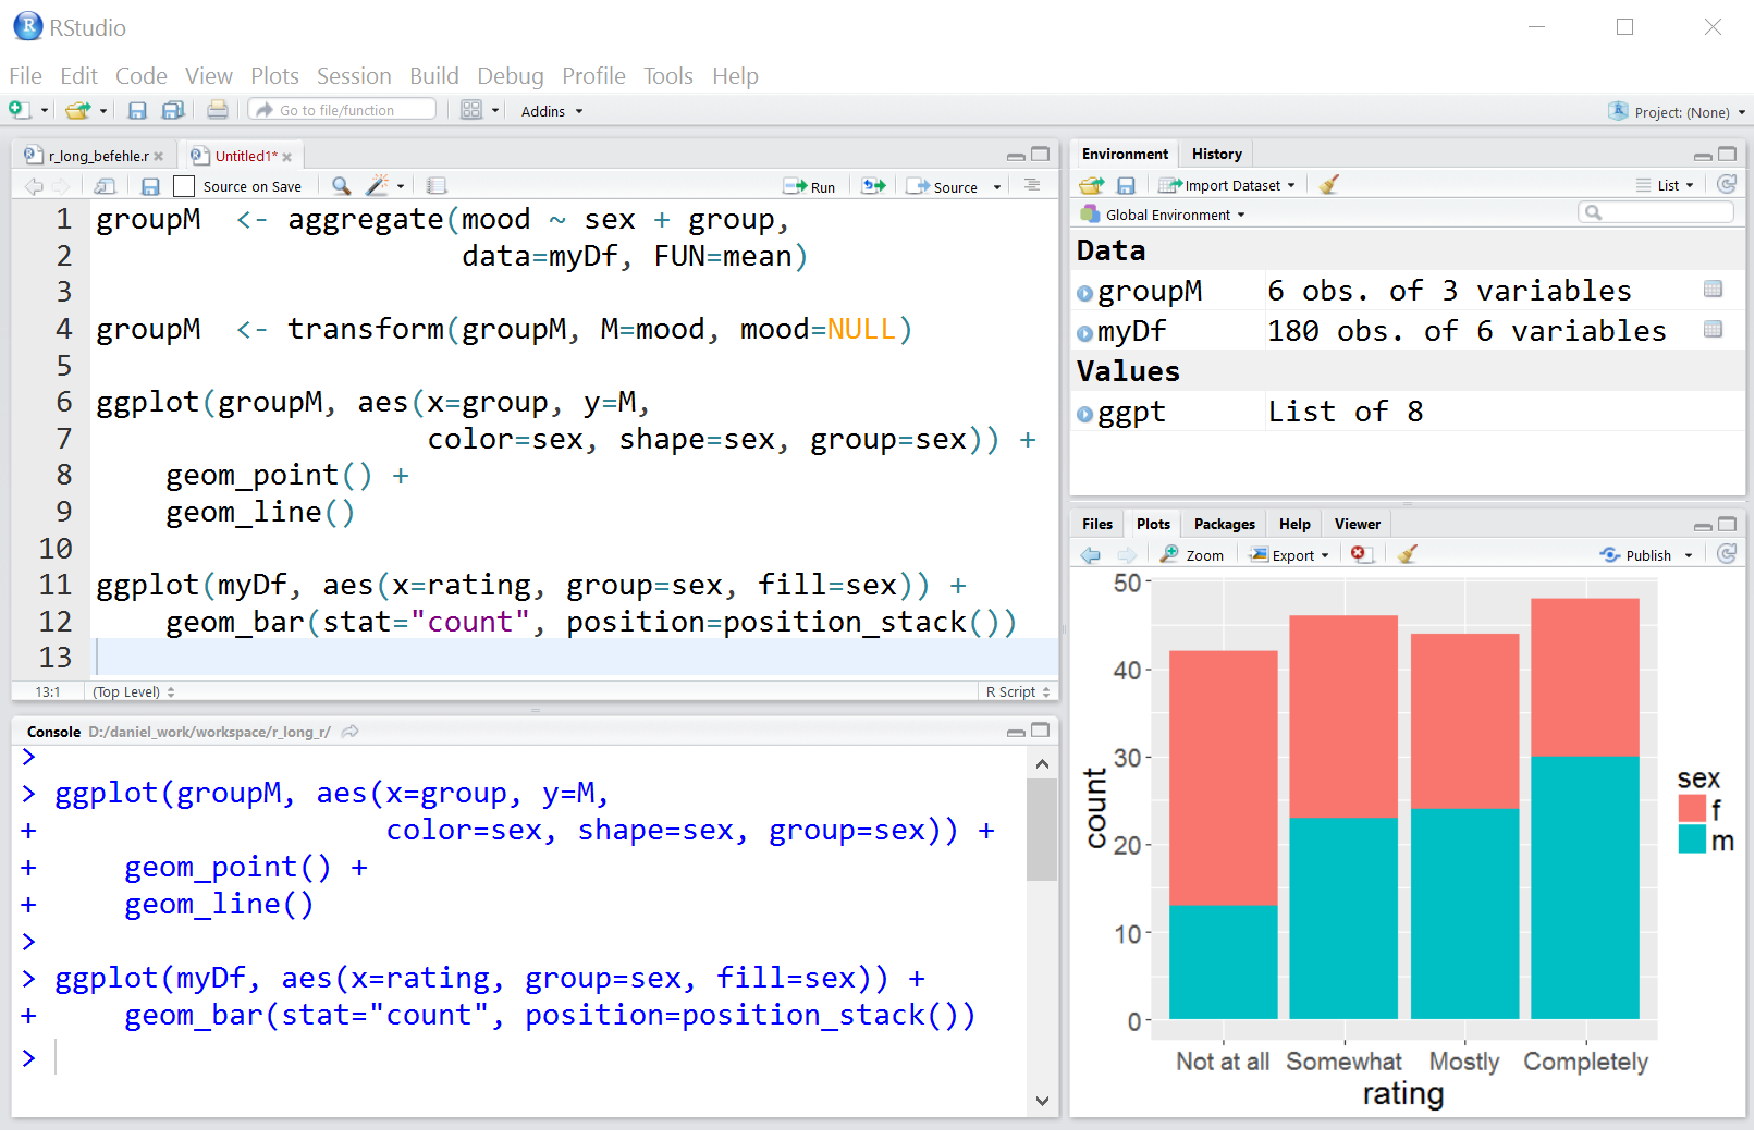
\includegraphics[width=12.5cm]{rstudio}
\vspace*{-0.5em}
\caption{Oberfläche der Entwicklungsumgebung RStudio}
\label{fig:rstudio}
\end{figure}

Auf der Konsole werden im interaktiven Wechsel von eingegebenen Befehlen und der Ausgabe von R die Verarbeitungsschritte vorgenommen.\footnote{Für automatisierte Auswertungen s.\ Abschn.\ \ref{sec:scripting}. Um die Ausgabe ganz oder als Protokoll-Kopie aller Vorgänge in eine Datei umzuleiten s.\ Abschn. \ref{sec:sink}. Befehle des Betriebssystems sind mit\index[func]{shell()@\lstinline{shell()}} \lstinline!shell("<<Befehl>>")! ausführbar, so können etwa die Netzwerkverbindungen mit \lstinline!shell("netstat")! angezeigt werden.} Hier erscheint nach dem Start unter einigen Hinweisen zur installierten R-Version hinter dem \emph{Prompt}-Zeichen\index{Prompt}\index[func]{>@\lstinline{>}} \lstinline!>! ein Cursor. Der Cursor signalisiert, dass Befehle vom Benutzer entgegengenommen und verarbeitet werden können. Das Ergebnis einer Berechnung wird in der auf das Prompt-Zeichen folgenden Zeile ausgegeben, nachdem ein Befehl mit der \myURL{Return} Taste beendet wurde. Dabei wird in eckigen Klammern oft zunächst die laufende Nummer des ersten in der jeweiligen Zeile angezeigten Objekts aufgeführt. Anschließend erscheint erneut ein Prompt-Zeichen, hinter dem neue Befehle eingegeben werden können.
\begin{lstlisting}
> 1 + 1
[1] 2

>
\end{lstlisting}

\index[func]{"\#@\texttt{\#}|textbf}
Pro Zeile wird im Normalfall ein Befehl eingegeben. Sollen mehrere Befehle in eine Zeile geschrieben werden, so sind sie durch ein\index[func]{;@\lstinline{;}} \lstinline!;! zu trennen. Das Symbol \lstinline!#! markiert den Beginn eines \emph{Kommentars}\index{Kommentar} und verhindert, dass der dahinter auftauchende Text in derselben Zeile als Befehl interpretiert wird.

War die Eingabe nicht korrekt, erscheint eine Fehlermeldung mit einer Beschreibung der Ursache. Abschnitt \ref{sec:mistakes} erläutert typische Fehlerquellen. Befehle können auch Warnungen verursachen, die die Auswertung zwar nicht wie Fehler verhindern, aber immer daraufhin untersucht werden sollten, ob sie ein Symptom für falsche Berechnungen sind.

Das folgende Beispiel demonstriert eine kurze Auswertung in Form mehrerer aufeinanderfolgender Arbeitsschritte. An dieser Stelle ist es dabei nicht wichtig, schon zu verstehen, wie die einzelnen Befehle funktionieren. Vielmehr soll das Beispiel zeigen, wie eine realistische Sequenz von Auswertungsschritten inkl.\ der von R erzeugten Ausgabe aussehen kann. Die Analyse bezieht sich auf den Datensatz \lstinline!Duncan! aus dem Paket \lstinline!carData!\index[pack]{carData@\lstinline{carData}|textbf} \cite{Fox2019}, das zunächst zu installieren ist (Abschn.\ \ref{sec:packages}). Der Datensatz speichert Daten von Personen verschiedener Berufe. Ein Beruf kann dabei zur Gruppe \lstinline!bc! (\emph{blue collar}), \lstinline!wc! (\emph{white collar}) oder \lstinline!prof! (\emph{professional}) gehören -- die Stufen der Variable \lstinline!type!. Erhoben wurde der prozentuale Anteil von Personen eines Berufs mit einem hohen Einkommen (Variable \lstinline!income!), einem hohen Ausbildungsgrad (\lstinline!education!) und einem hohen Prestige (\lstinline!prestige!). Jede Zeile enthält die Daten jeweils eines Berufs, die Daten jeweils einer Variable finden sich in den Spalten des Datensatzes.

\begin{lstlisting}
> data(Duncan, package="carData") # lade Datensatz Duncan aus carData
> head(Duncan, n=4)               # die ersten 4 Zeilen von Duncan
            type  income  education  prestige
accountant  prof      62         86        82
pilot       prof      72         76        83
architect   prof      75         92        90
author      prof      55         90        76
\end{lstlisting}

Zunächst sollen wichtige deskriptive Kennwerte von \lstinline!income! in nach Gruppen getrennten \emph{boxplots} dargestellt und dabei auch die Rohdaten selbst abgebildet werden (Abb.\ \ref{fig:duncanBox}). Es folgt die Berechnung der Gruppenmittelwerte für \lstinline!education! und die Korrelationsmatrix der drei erhobenen Variablen. Als inferenzstatistische Auswertung schließt sich eine Varianzanalyse mit der Variable \lstinline!prestige! und dem Gruppierungsfaktor \lstinline!type! an. Im folgenden $t$-Test der Variable \lstinline!education! sollen nur die Gruppen \lstinline!bc! und \lstinline!wc! berücksichtigt werden.
\begin{lstlisting}
# nach Gruppen getrennte boxplots und Rohdaten der Variable income
> boxplot(income ~ type, data=Duncan,
+         main="Anteil hoher Einkommen pro Berufsgruppe")

> stripchart(income ~ type, data=Duncan, pch=20, vert=TRUE, add=TRUE)

#####
# Gruppenmittelwerte von income und education getrennt nach type
> aggregate(cbind(income, education) ~ type, FUN=mean, data=Duncan)
  type   income education
1   bc 23.76190  25.33333
2 prof 60.05556  81.33333
3   wc 50.66667  61.50000

#####
# Korrelationsmatrix der Variablen income, education, prestige
> with(Duncan, cor(cbind(income, education, prestige)))
              income  education   prestige
income     1.0000000  0.7245124  0.8378014
education  0.7245124  1.0000000  0.8519156
prestige   0.8378014  0.8519156  1.0000000

#####
# einfaktorielle Varianzanalyse von prestige in Gruppen type
> anova(lm(prestige ~ type, data=Duncan))
Analysis of Variance Table
Response: prestige
           Df  Sum Sq  Mean Sq  F value     Pr(>F)
type        2   33090    16545   65.571  1.207e-13 ***
Residuals  42   10598      252

#####
# nur Berufe der Gruppen bc oder wc auswählen
> BCandWC <- with(Duncan, (type == "bc") | (type == "wc"))

#####
# linksseitiger t-Test der Variable education
# für die zwei ausgewählten Berufsgruppen bc und wc
> t.test(education ~ type,
+        alternative="less", data=Duncan, subset=BCandWC)
Welch Two Sample t-test
data:  education by type
t = -4.564, df = 5.586, p-value = 0.002293
alternative hypothesis: true difference in means is less than 0
95 percent confidence interval:
      -Inf -20.56169

sample estimates:
mean in group bc  mean in group wc
        25.33333          61.50000
\end{lstlisting}

\begin{figure}[ht]
\centering
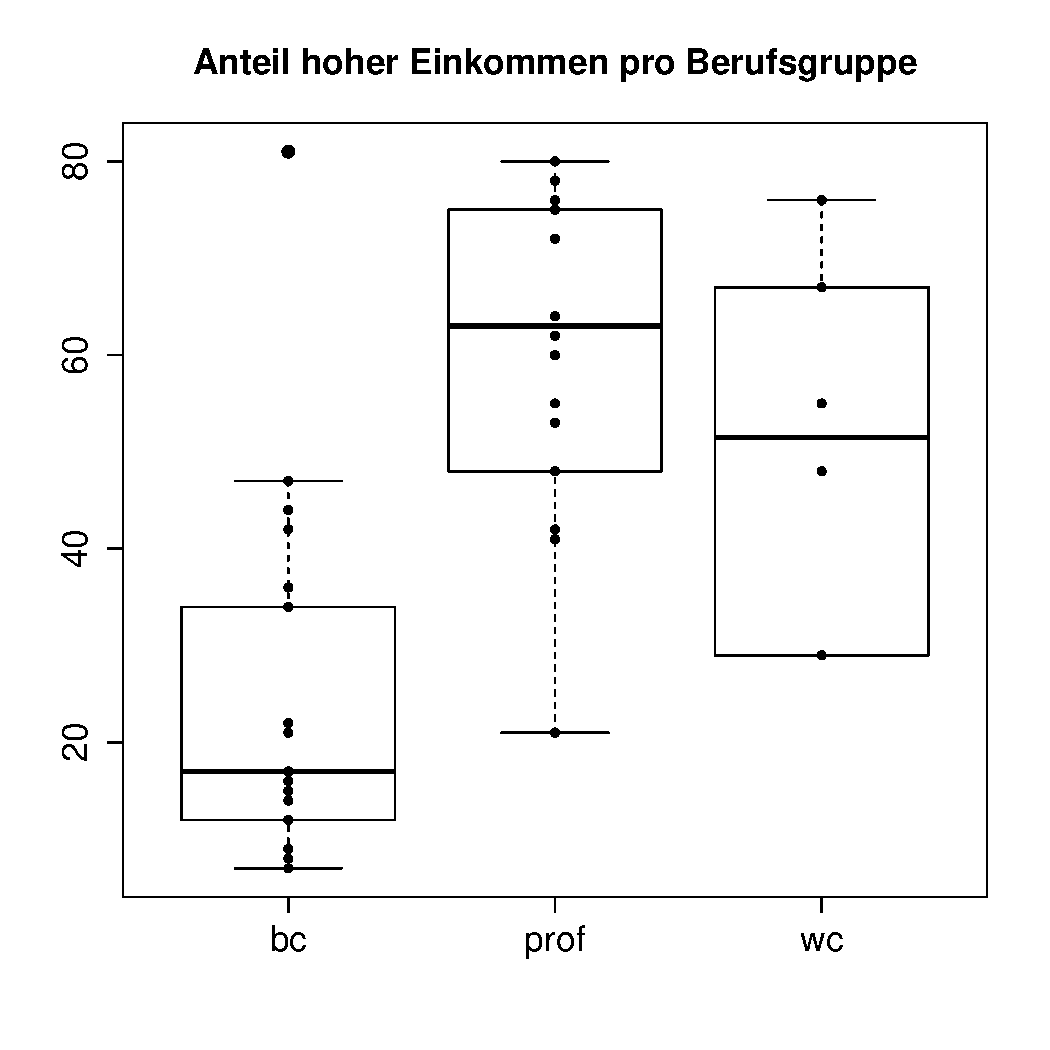
\includegraphics[width=8cm]{duncanBox}
\vspace*{-1em}
\caption{Daten des Datensatzes \lstinline!Duncan!: Anteil der Angehörigen eines Berufs mit hohem Einkommen in Abhängigkeit vom Typ des Berufs}
\label{fig:duncanBox}
\end{figure}

Einzelne Befehlsbestandteile müssen meist nicht unbedingt durch Leerzeichen getrennt werden, allerdings erhöht dies die Übersichtlichkeit und ist mitunter auch erforderlich. Insbesondere das Zuweisungssymbol \lstinline!<-! sollte stets von Leerzeichen umschlossen sein. Wenn ein Befehl die sichtbare Zeilenlänge der Konsole überschreitet, verlängert R die Zeile automatisch, schränkt aber auf diese Weise die Sichtbarkeit des Befehlsbeginns ein. Ein langer Befehl kann darum auch durch Drücken der \myURL{Return} Taste in der nächsten Zeile fortgesetzt werden, solange er syntaktisch nicht vollständig ist -- z.\,B.\ wenn eine geöffnete Klammer noch nicht geschlossen wurde. Es erscheint dann ein\index[func]{+@\lstinline{+}} \lstinline!+! zu Beginn der folgenden Zeile, um zu signalisieren, dass sie zur vorangehenden gehört. Falls dieses \lstinline!+! ungewollt in der Konsole auftaucht, muss der Befehl entweder vervollständigt oder mit der \myURL{ESC} Taste\index{Tastaturkurzel@Tastaturkürzel} (Windows) bzw.\ der \myURL{Strg+c} Tastenkombination (Linux) abgebrochen werden.
\begin{lstlisting}
> 2 * (4
+ -5)
[1] -2
\end{lstlisting}

In der Konsole können Befehle mit der Maus markiert und (unter Windows) über die Tastenkombination \myURL{Strg+c} in die Zwischenablage hinein bzw.\ mit \myURL{Strg+v} aus der Zwischenablage heraus in die Befehlszeile hinein kopiert werden.

Wird der Anfang eines Befehlsnamens in der Konsole oder im Editor eingegeben, bietet RStudio mit einer kurzen Zeitverzögerung automatisch mögliche Vervollständigungen des begonnenen Befehls an. In der Konsole des Basisumfangs von R ist dafür zweimal die Tabulator-Taste zu drücken. Es existieren noch weitere vergleichbare Kurzbefehle, über die das RStudio Menü \emph{Help: Keyboard Shortcuts} informiert.

\index{beenden}
R wird entweder über den Befehl\index[func]{q()@\lstinline{q()}} \lstinline!q()! in der Konsole, über den Menüpunkt \emph{File: Quit RStudio} oder durch Schließen des Programmfensters beendet. Zuvor erscheint die Frage, ob man den \emph{workspace}, also alle erstellten Daten, im aktuellen Arbeitsverzeichnis speichern möchte (Abschn.\ \ref{sec:settings}, \ref{sec:workspace}).

%%%%%%%%%%%%%%%%%%%%%%%%%%%%%%%%%%%%%%%%%%%%%%%%%%%%%%%%%%%%%%%%%%
%%%%%%%%%%%%%%%%%%%%%%%%%%%%%%%%%%%%%%%%%%%%%%%%%%%%%%%%%%%%%%%%%%
\subsection{Einstellungen}
\label{sec:settings}
%%%%%%%%%%%%%%%%%%%%%%%%%%%%%%%%%%%%%%%%%%%%%%%%%%%%%%%%%%%%%%%%%%
%%%%%%%%%%%%%%%%%%%%%%%%%%%%%%%%%%%%%%%%%%%%%%%%%%%%%%%%%%%%%%%%%%

\index{Einstellungen}
\index{Verzeichnis!Arbeitsverzeichnis}
\index{Arbeitsverzeichnis|see{Verzeichnis}}
\index{Ordner|see{Verzeichnis}}
R wird immer in einem \emph{Arbeitsverzeichnis} ausgeführt, das sich durch\index[func]{getwd()@\lstinline{getwd()}} \lstinline!getwd()! ausgeben lässt. In der Voreinstellung handelt es sich um das Heimverzeichnis des Benutzers, das man mit\index[func]{path.expand()@\lstinline{path.expand()}} \lstinline!path.expand("~")! erfährt. Alle während einer Sitzung gespeicherten Dateien werden, sofern nicht explizit anders angegeben, in diesem Verzeichnis abgelegt. Wenn Informationen aus Dateien geladen werden sollen, greift R ebenfalls auf dieses Verzeichnis zu, sofern kein anderes ausdrücklich genannt wird. Um das voreingestellte Arbeitsverzeichnis zu ändern, existieren folgende Möglichkeiten:

\begin{itemize}
\item Unter Windows durch einen Rechtsklick auf die auf dem desktop erstellte Verknüpfung mit R: \emph{Eigenschaften} auswählen und anschließend bei \emph{Ausführen in} ein neues Arbeitsverzeichnis angeben. Dies führt dazu, dass R von nun an immer im angegebenen Arbeitsverzeichnis startet, wenn die Verknüpfung zum Programmstart verwendet wird.
\item Im Menü der R-eigenen Oberfläche unter Windows kann \emph{Datei} \textrightarrow\ \emph{Verzeichnis wechseln} gewählt und anschließend ein neues Arbeitsverzeichnis angegeben werden. Dieser Schritt ist dann nach jedem Start von R zu wiederholen. Eine analoge Funktion findet sich in RStudio im Menüpunkt \emph{Session} \textrightarrow\ \emph{Set Working Directory}.
\item In der Konsole lässt sich das aktuelle Arbeitsverzeichnis mit\index[func]{setwd()@\lstinline{setwd()}} \lstinline!setwd("<<Pfad>>")! ändern, unter Windows also z.\,B.\ mit \lstinline!setwd("c:/work/r/")! (s.\ Abschn.\ \ref{sec:files} für die möglichen Formen von Pfadangaben).
\end{itemize}

\index{Optionen}
\index{anpassen|see{Optionen}}
R wird mit einer Reihe von Voreinstellungen gestartet, die sich über selbst editierbare Textdateien steuern lassen, über die \lstinline!?Startup! Auskunft gibt \cite{RDevelopmentCoreTeam2008a}. Sollen etwa bestimmte Pakete in jeder Sitzung geladen werden (Abschn.\ \ref{sec:packages}), können die entsprechenden \lstinline!library()! Befehle in die Datei\index[func]{Rprofile.site@\myURL{Rprofile.site}} \myURL{Rprofile.site} im \myURL{etc/} Ordner des Programmordners geschrieben werden.\footnote{Zudem kann jeder Benutzer eines Computers dazu die Datei\index[func]{.Rprofile@\myURL{.Rprofile}} \myURL{.Rprofile} in seinem Heimverzeichnis anlegen. In dieser Datei können auch die Funktionen namens\index[func]{.First()@\lstinline{.First()}}\index[func]{.Last()@\lstinline{.Last()}} \lstinline!.First! bzw.\ \lstinline!.Last! mit beliebigen Befehlen definiert werden, die dann beim Start als erstes bzw.\ beim Beenden als letztes ausgeführt werden (Abschn.\ \ref{sec:function}). R auf diesem Weg individuell zu konfigurieren, senkt jedoch die Reproduzierbarkeit der Auswertungen (Abschn.\ \ref{sec:reproducibility}).} Gleiches gilt für befehlsübergreifende Voreinstellungen, die mit\index[func]{getOption()@\lstinline{getOption()}} \lstinline!getOption()! angezeigt und mit \index[func]{options()@\lstinline{options()}|textbf} \lstinline!options()! verändert werden können.
\begin{lstlisting}
getOption("<<Option>>")        # gibt aktuellen Wert für <<Option>> aus
options(<<Option>>=<<Wert>>)     # setzt <<Option>> auf <<Wert>>
\end{lstlisting}

Mit \lstinline!options(width=<<Anzahl>>)! kann z.\,B.\ festgelegt werden, mit wie vielen Zeichen pro Zeile die Ausgabe von R erfolgt. \lstinline!options()! liefert dabei auf der Konsole unsichtbar den Wert zurück, den die Einstellung vor ihrer Änderung hatte. Wird dieser Wert in einem Objekt gespeichert, kann die Einstellung später wieder auf ihren ursprünglichen Wert zurückgesetzt werden.
\begin{lstlisting}
> getOption("width")      # aktuellen Wert für Option anzeigen
[1] 116

> op <- options(width=70) # Option ändern & alten Wert in op speichern
> options(op)             # Option auf alten Wert zurücksetzen
\end{lstlisting}

%%%%%%%%%%%%%%%%%%%%%%%%%%%%%%%%%%%%%%%%%%%%%%%%%%%%%%%%%%%%%%%%%%
%%%%%%%%%%%%%%%%%%%%%%%%%%%%%%%%%%%%%%%%%%%%%%%%%%%%%%%%%%%%%%%%%%
\subsection{Umgang mit dem workspace}
\label{sec:workspace}
%%%%%%%%%%%%%%%%%%%%%%%%%%%%%%%%%%%%%%%%%%%%%%%%%%%%%%%%%%%%%%%%%%
%%%%%%%%%%%%%%%%%%%%%%%%%%%%%%%%%%%%%%%%%%%%%%%%%%%%%%%%%%%%%%%%%%

\index{workspace}
R speichert automatisch temporär alle während einer Sitzung ausgeführten Befehle und neu erstellten Daten. Die Daten liegen dabei in einem\index{Umgebung}\index{environment|see{Umgebung}} \emph{workspace}, der auch als \emph{Umgebung} (\emph{environment}) bezeichnet wird. So können Kopien von Befehlen und Daten nachträglich in externen Dateien abgespeichert und bei einer neuen Sitzung wieder genutzt werden. Auf bereits eingegebene Befehle kann auch bereits während derselben Sitzung erneut zugegriffen werden: Über die Pfeiltasten nach oben und unten lassen sich verwendete Befehle wieder aufrufen. Diese Funktion wird im Folgenden als Befehlshistorie\index{Befehlshistorie} bezeichnet. Eine Übersicht der letzten Befehle liefert die Funktion\index[func]{history()@\lstinline{history()}} \lstinline!history()!, in RStudio finden sich die Befehle im Tab \emph{History}.

Der erwähnte workspace trägt den Namen \index[func]{.GlobalEnv@\lstinline{.GlobalEnv}} \lstinline!.GlobalEnv!. Neben ihm existieren noch weitere Umgebungen, die abgekapselt voneinander ebenfalls Objekte speichern. Da ein Nutzer auf die Objekte aller Umgebungen zugreifen kann, tritt dieser Umstand nur selten explizit zutage, ist jedoch manchmal wichtig: Objekte, die in unterschiedlichen Umgebungen liegen, können denselben Namen tragen, ohne dass ihre Inhalte wechselseitig überschrieben würden (Abschn.\ \ref{sec:objectNames}). Die Umgebungen sind intern linear geordnet. Die Reihenfolge, in der R die Umgebungen nach Objekten durchsucht, ist der\index{Suchpfad} \emph{Suchpfad}, der von \index[func]{search()@\lstinline{search()}} \lstinline!search()! ausgegeben wird. Existieren mehrere Objekte desselben Namens in unterschiedlichen Umgebungen, bezeichnet der einfache Name das Objekt in der früheren Umgebung. Welche Objekte eine bestimmte Umgebung speichert, lässt sich auf der Konsole mit\index[func]{ls()@\lstinline{ls()}} \lstinline!ls()! feststellen, während RStudio dafür den \emph{Environment} Tab besitzt.
\begin{lstlisting}
ls(name="<<Umgebung>>", pattern="<<Suchmuster>>")
\end{lstlisting}

In der Voreinstellung \lstinline!ls()! werden die Objekte der derzeit aktiven Umgebung aufgelistet, bei einem Aufruf von der Konsole i.\,d.\,R.\ also jene aus \lstinline!.GlobalEnv!, der ersten Umgebung im Suchpfad. Alternativ kann für \lstinline!name! der Name einer Umgebung oder aber ihre Position im Suchpfad angegeben werden. Über \lstinline!pattern! lässt sich ein Muster für den Objektnamen spezifizieren, so dass nur solche Objekte angezeigt werden, deren Name auf das Muster passt. Im einfachsten Fall könnte das Muster ein Buchstabe sein, den der Objektname enthalten muss, kompliziertere Muster sind über \emph{reguläre Ausdrücke} möglich (Abschn.\ \ref{sec:grep}).
\begin{lstlisting}
> ls()                      # nenne alle Objekte der aktuellen Umgebung
[1] "BCandWC" "Duncan"

# Objekte der Standard-Umgebung, die ein großes C im Namen tragen
> ls(".GlobalEnv", pattern="C")
[1] "BCandWC"
\end{lstlisting}

Es gibt mehrere, in ihren Konsequenzen unterschiedliche Wege, Befehle und Daten der aktuellen Sitzung zu\index{speichern|see{workspace}} sichern. Eine Kopie des aktuellen workspace sowie der Befehlshistorie wird etwa gespeichert, indem man die beim Beenden von R erscheinende diesbezügliche Frage bejaht. Als Folge wird -- falls vorhanden -- der sich in diesem Verzeichnis befindende, bereits während einer früheren Sitzung gespeicherte workspace automatisch überschrieben. R legt bei diesem Vorgehen zwei Dateien an: eine, die lediglich die erzeugten Daten der Sitzung enthält (Datei\index[func]{.RData@\lstinline[language=]{.RData}} \lstinline[language=]{.RData}) und eine mit der Befehlshistorie (Datei\index[func]{.Rhistory@\lstinline[language=]{.Rhistory}} \lstinline[language=]{.Rhistory}). Der so gespeicherte workspace wird beim nächsten Start von R automatisch geladen.

Da es im Sinne der Reproduzierbarkeit der Auswertungsumgebung sinnvoller ist, immer mit einem leeren workspace zu starten und Objekte dann explizit zu erstellen (Abschn.\ \ref{sec:reproducibility}), sollte die Frage nach einer Sicherung der Sitzung verneint werden. In RStudio verhindern dies entsprechende Einstellungen im Menü \emph{Tools} \textrightarrow\ \emph{Global Options...} \textrightarrow\ \emph{R General} \textrightarrow\ \emph{Workspace} dauerhaft.

Der workspace kann in RStudio im \emph{Environment} Tab über das Disketten-icon unter einem frei wählbaren Namen gespeichert werden, um früher angelegte Dateien nicht zu überschreiben. Über das Ordner-icon im \emph{Environment} Tab lässt sich eine Workspace-Datei wieder laden. Dabei ist zu beachten, dass zuvor definierte Objekte von jenen Objekten aus dem geladenen workspace überschrieben werden, die denselben Namen tragen. Die manuell gespeicherten workspaces werden bei einem Neustart von R nicht automatisch geladen.

Um die Befehlshistorie unter einem bestimmten Dateinamen abzuspeichern, wählt man den \emph{History} Tab, der ebenfalls ein Disketten-icon besitzt. In der Konsole stehen zum Speichern und Laden der Befehlshistorie die Funktionen\index[func]{savehistory()@\lstinline{savehistory()}} \lstinline!savehistory("<<Dateiname>>")! und\index[func]{loadhistory()@\lstinline{loadhistory()}} \lstinline!loadhistory("<<Dateiname>>")! zur Verfügung.

%%%%%%%%%%%%%%%%%%%%%%%%%%%%%%%%%%%%%%%%%%%%%%%%%%%%%%%%%%%%%%%%%%
%%%%%%%%%%%%%%%%%%%%%%%%%%%%%%%%%%%%%%%%%%%%%%%%%%%%%%%%%%%%%%%%%%
\subsection{Einfache Arithmetik}
\label{sec:arithmetic}
%%%%%%%%%%%%%%%%%%%%%%%%%%%%%%%%%%%%%%%%%%%%%%%%%%%%%%%%%%%%%%%%%%
%%%%%%%%%%%%%%%%%%%%%%%%%%%%%%%%%%%%%%%%%%%%%%%%%%%%%%%%%%%%%%%%%%

\index{Arithmetik}
\index{Operatoren}
\index{Konstanten}
\index{Zahlen!Grundrechenarten}
In R sind die grundlegenden arithmetischen Operatoren, Funktionen und Konstanten implementiert, über die auch ein Taschenrechner verfügt. Für eine Übersicht vgl.\ die mit \lstinline!?Syntax! und \lstinline!?Arithmetic! aufzurufenden Hilfe-Seiten. Punktrechnung geht dabei vor Strichrechnung, das Dezimaltrennzeichen\index{Zahlen!Dezimaltrennzeichen|textbf} ist unabhängig von den Ländereinstellungen des Betriebssystems immer der Punkt. Nicht ganzzahlige Werte werden in der Voreinstellung mit sieben relevanten Stellen\index{Zahlen!Dezimalstellen} ausgegeben, was mit dem Befehl\index[func]{options()@\lstinline{options()}} \lstinline!options(digits=<<Anzahl>>)! veränderbar ist.

Alternativ können Zahlen auch in wissenschaftlicher, also verkürzter Exponentialschreibweise\index{Zahlen!Exponentialschreibweise} ausgegeben werden.\footnote{Sofern diese Formatierung nicht mit\index[func]{options()@\lstinline{options()}} \lstinline!options(scipen=999)! ganz unterbunden wird. Allgemein kann dabei mit ganzzahlig positiven Werten für \lstinline!scipen! (\emph{scientific penalty}) die Schwelle erhöht werden, ab der R die wissenschaftliche Notation für Zahlen verwendet (vgl.\ \lstinline!?options!).} Dabei ist z.\,B.\ der Wert \lstinline!2e-03! als $2 \cdot 10^{-3}$, also $\frac{2}{10^{3}}$, mithin $0.002$ zu lesen. Auch die Eingabe von Zahlen ist in diesem Format möglich.

%\begin{tabular*}{0.75\textwidth}{@{\extracolsep{\fill}} | c | c | c | r | }
\begin{longtable}{p{5.1cm}p{7.4cm}}
\caption{Arithmetische Funktionen, Operatoren und Konstanten
\label{tab:funcOperatorConst}}\\
\endfirsthead
\caption[]{(Forts.)}\\\hline
\endhead
\hline
\sffamily Name & \sffamily Bedeutung\\\hline\hline
\lstinline!+! , \lstinline!-! \index[func]{+@\lstinline{+}} \index[func]{-@\lstinline{-}} & Addition, Subtraktion\\
\lstinline!*! , \lstinline!/! \index[func]{*@\lstinline{*}} \index[func]{/@\lstinline{/}} & Multiplikation, Division\\
\lstinline!%/%! \index[func]{\%/\%@\texttt{\%/\%}} & ganzzahlige Division (ganzzahliges Ergebnis einer Division ohne Rest)\\
\lstinline!%%! \index[func]{\%\%@\texttt{\%\%}} & Modulo Division (Rest einer ganzzahligen Division, verallgemeinert auf Dezimalzahlen\footnote{Der Dezimalteil \index{Zahlen!Dezimalteil} einer Dezimalzahl ergibt sich also als \lstinline!<<Zahl>> \%\% 1!.})\\
\lstinline!^! \index[func]{^@\lstinline{^}|textbf} & potenzieren\\
\lstinline!sign()! \index[func]{sign()@\lstinline{sign()}} & Vorzeichen \index{Zahlen!Vorzeichen} (\lstinline!-1! bei negativen, \lstinline!1! bei positiven Zahlen, \lstinline!0! bei der Zahl $0$)\\
\lstinline!abs()! \index[func]{abs()@\lstinline{abs()}} & Betrag\index{Zahlen!Betrag}\\
\lstinline!sqrt()! \index[func]{sqrt()@\lstinline{sqrt()}} & Quadratwurzel\index{Zahlen!Quadratwurzel}\\
\lstinline!round()! \index[func]{round()@\lstinline{round()}} \index{Zahlen!runden} & runden (mit Argument \lstinline!digits! zur Anzahl der Dezimalstellen)\footnote{R rundet in der Voreinstellung nicht nach dem vielleicht vertrauten Prinzip des kaufmännischen Rundens, sondern \emph{unverzerrt} \cite{Bronstein2008}. Durch negative Werte für \lstinline!digits! kann auch auf Zehnerpotenzen gerundet werden. \lstinline!signif()! rundet\index[func]{signif()@\lstinline{signif()}} auf eine bestimmte Anzahl signifikanter Stellen.}\\
\lstinline!floor()!, \lstinline!ceiling()!, \lstinline!trunc()! \index[func]{floor()@\lstinline{floor()}} \index[func]{ceiling()@\lstinline{ceiling()}}
\index[func]{trunc()@\lstinline{trunc()}} & auf nächsten ganzzahligen Wert \index{Zahlen!runden} abrunden, aufrunden, tranchieren (Nachkommastellen abschneiden)\\
\lstinline!log()!, \lstinline!log10()!, \lstinline!log2()!, \lstinline[breaklines=false]!log(<<Zahl>>, base=<<Basis>>)! \index[func]{log()@\lstinline{log(), log2(), log10()}} & natürlicher \index{Zahlen!Logarithmus} Logarithmus, Logarithmus zur Basis $10$, zur Basis $2$, zu beliebiger Basis\\
\lstinline!exp()!\index[func]{exp()@\lstinline{exp()}} & Exponentialfunktion\index{Exponentialfunktion}\\
\lstinline!exp(1)! & Eulersche Zahl \index{Zahlen!e@$\euler$} $\euler$\\
\lstinline!sin()!, \lstinline!cos()!, \lstinline!tan()!, \lstinline!asin()!, \lstinline[breaklines=false]!acos()!, \lstinline!atan()!, \lstinline!atan2()! \index[func]{sin()@\lstinline{sin()}} \index[func]{cos()@\lstinline{cos()}} \index[func]{tan()@\lstinline{tan()}} \index[func]{asin()@\lstinline{asin()}} \index[func]{acos()@\lstinline{acos()}} \index[func]{atan()@\lstinline{atan()}} \index[func]{atan2()@\lstinline{atan2()}} & trigonometrische Funktionen \index{trigonometrische Funktionen} \index{Winkelfunktionen|see{trigonometrische Funktionen}} sowie ihre Umkehrfunktionen (Argument im Bogenmaß)\\
\lstinline!factorial()! \index[func]{factorial()@\lstinline{factorial()}} \index{Zahlen!Fakultät} & Fakultät\\
\lstinline!pi! \index[func]{pi@\lstinline{pi}} \index{Zahlen!PI@$\pi$} & Kreiszahl $\pi$\\
\lstinline!Inf!, \lstinline!-Inf! \index[func]{Inf@\lstinline{Inf}} & $\infty, -\infty$ \index{Zahlen!unendlich} (\emph{infinity})\\
\lstinline!NA! \index[func]{NA@\lstinline{NA}} & fehlender Wert \index{Daten!fehlende Werte} (\emph{not available})\\
\lstinline!NaN! \index[func]{NaN@\lstinline{NaN}} & nicht definiert (\emph{not a number}), verhält sich weitestgehend wie \lstinline!NA!\\
\lstinline!NULL! \index[func]{NULL@\lstinline{NULL}} & leere Menge\index{leere Menge}\\\hline
\end{longtable}

Die in Tab.\ \ref{tab:funcOperatorConst} aufgeführten Funktionen, Operatoren und Konstanten sind frei kombinierbar und können auch ineinander verschachtelt werden. Um die Reihenfolge der Auswertung eindeutig zu halten, sollten in Zweifelsfällen\index{Klammern} Klammern gesetzt werden.\footnote{Für die zur Bestimmung der Ausführungsreihenfolge wichtige\index{Assoziativitat@Assoziativität}\index{Ausführungsreihenfolge|see{Assoziativität}} Assoziativität von Operatoren vgl.\ \lstinline!?Syntax!.}
\begin{lstlisting}
> 12^2 + 1.5*10
[1] 159

> sin(pi/2) + sqrt(abs(-4))
[1] 3
\end{lstlisting}

\lstinline!<<Realteil>>+<<Imaginärteil>>i! ist die Notation zur Eingabe\index{Zahlen!komplexe}\index{komplexe Zahlen|see{Zahlen}} komplexer Zahlen. \lstinline!0+1i! ist also die imaginäre Zahl\index{Zahlen!i@$i$} $i$, \lstinline!-1+0i! hingegen die reelle Zahl $-1$ in komplexer Schreibweise. Den Realteil einer komplexen Zahl liefert\index[func]{Re()@\lstinline{Re()}} \lstinline!Re(<<Zahl>>)!, den Imaginärteil\index[func]{Im()@\lstinline{Im()}} \lstinline!Im(<<Zahl>>)!. Die Funktionen\index[func]{Mod()@\lstinline{Mod()}} \lstinline!Mod(<<Zahl>>)! und\index[func]{Arg()@\lstinline{Arg()}} \lstinline!Arg(<<Zahl>>)! geben die Polarkoordinaten in der komplexen Ebene aus, die komplex Konjugierte ermittelt \index[func]{Conj()@\lstinline{Conj()}} \lstinline!Conj(<<Zahl>>)!. In der Voreinstellung rechnet R mit reellen Zahlen, aus diesem Grund erzeugt etwa \lstinline!sqrt(-1)! die Ausgabe \lstinline!NaN!, während \lstinline!sqrt(-1+0i)! mit \lstinline!0+1i! das richtige Ergebnis $i$ liefert.
\begin{lstlisting}
> exp(1)^((0+1i) * pi)            # komplexe Zahl (Eulersche Identität)
[1] -1+0i
\end{lstlisting}

\index[func]{is.infinite()@\lstinline{is.infinite()}}
\index[func]{is.finite()@\lstinline{is.finite()}}
\index[func]{is.nan()@\lstinline{is.nan()}}
\index[func]{is.na()@\lstinline{is.na()}}
\index[func]{is.null()@\lstinline{is.null()}}
Um zu überprüfen, ob ein Objekt einen {\quotedblbase}besonderen{\textquotedblleft} numerischen Wert speichert, stellt R Funktionen bereit, die nach dem Muster \lstinline!is.<<Prüfwert>>(<<Zahl>>)! aufgebaut sind und einen Wahrheitswert zurückgeben (Abschn.\ \ref{sec:isTRUE}).
\begin{lstlisting}
is.infinite(<<Zahl>>)            # ist <<Zahl>> +/- unendlich?
is.finite(<<Zahl>>)              # ist <<Zahl>> gültige endliche Zahl?
is.nan(<<Zahl>>)                 # ist <<Zahl>> nicht definiert?
is.na(<<Zahl>>)                  # ist <<Zahl>> ein fehlender Wert?
is.null(<<Zahl>>)                # ist <<Zahl>> die leere Menge?
\end{lstlisting}

\begin{lstlisting}
> is.infinite(1/0)
[1] TRUE

> is.nan(0/0)
[1] TRUE
\end{lstlisting}

Die Funktion \lstinline!is.finite(<<Objekt>>)! liefert nur für solche Objekte \lstinline!TRUE! zurück, die eine gültige Zahl sind, neben \lstinline!-Inf! und \lstinline!Inf! ergeben auch Zeichenketten, \lstinline!NA!, \lstinline!NaN! und \lstinline!NULL! das Ergebnis \lstinline!FALSE!.

%%%%%%%%%%%%%%%%%%%%%%%%%%%%%%%%%%%%%%%%%%%%%%%%%%%%%%%%%%%%%%%%%%
%%%%%%%%%%%%%%%%%%%%%%%%%%%%%%%%%%%%%%%%%%%%%%%%%%%%%%%%%%%%%%%%%%
\subsection{Funktionen mit Argumenten aufrufen}
\label{sec:funcParam}
%%%%%%%%%%%%%%%%%%%%%%%%%%%%%%%%%%%%%%%%%%%%%%%%%%%%%%%%%%%%%%%%%%
%%%%%%%%%%%%%%%%%%%%%%%%%%%%%%%%%%%%%%%%%%%%%%%%%%%%%%%%%%%%%%%%%%

\index{Funktion!Argumente}
\index{Funktion!aufrufen}
Beim Aufruf von Funktionen in R sind die Werte, die der Funktion als notwendige Eingangsinformation dienen, in runde Klammern einzuschließen: \lstinline!<<Funktionsname>>(<<Argumentliste>>)!. Die Argumentliste besteht aus Zuweisungen an Argumente in der Form \lstinline!<<Argumentname>>=<<Wert>>!. Es können je nach Funktion ein oder mehrere durch Komma getrennte Argumente angegeben werden, die ihrerseits obligatorisch oder nur optional sein können.\footnote{In diesem Text werden nur die wichtigsten Argumente der behandelten Funktionen vorgestellt, eine vollständige Übersicht liefert jeweils\index[func]{args()@\lstinline{args()}} \lstinline!args(<<Funktionsname>>)! sowie die zugehörige Hilfe-Seite \lstinline!?<<Funktionsname>>!.} Auch wenn eine Funktion keine Argumente besitzt, müssen die runden Klammern vorhanden sein, z.\,B.\ \lstinline!q()!.\footnote{\label{ftn:functional}In R sind Operatoren wie \lstinline!+!, \lstinline!-!, \lstinline!*! oder \lstinline!/! Funktionen, für die lediglich eine bequemere und vertrautere Kurzschreibweise zur Verfügung steht. Operatoren lassen sich auch in der Präfix-Form benutzen, wenn sie in Anführungszeichen gesetzt werden. So ist \lstinline!\"/\"(1, 10)! äquivalent zu \lstinline!1/10!.}

Argumente sind benannt und machen so ihre Bedeutung für die Arbeitsweise der Funktion deutlich. Um z.\,B.\ eine Zahl zu runden, muss der Funktion \lstinline!round(<<Zahlen>>, digits=0)! mindestens ein zu rundender Wert übergeben werden, z.\,B.\ \lstinline!round(1.27)!. Weiterhin besteht die Möglichkeit, über das zusätzliche Argument \lstinline!digits! die gewünschte Anzahl an Nachkommastellen zu bestimmen: Mit \lstinline!round(pi, digits=2)! wird die Zahl $\pi$ auf zwei Dezimalstellen gerundet. Das\index{Funktion!Argumente} Argument \lstinline!digits! ist optional, wird es nicht angegeben, kommt der auf \lstinline!0! voreingestellte Wert (\emph{default}) zur Rundung auf ganze Zahlen zum tragen.

Der Name von Argumenten muss nicht unbedingt vollständig angegeben werden, wenn eine Funktion aufgerufen wird -- Kürzung auf den zur eindeutigen Identifizierung notwendigen Namensanfang reicht aus.\footnote{Gleiches gilt für die Werte von Argumenten, sofern sie aus einer festen Liste von Zeichenketten stammen. Statt \lstinline!cov(<<Matrix>>, use=\"pairwise.complete.obs\")! ist also auch \lstinline!cov(<<Matrix>>, u=\"pairwise\")! als Funktionsaufruf möglich.} Von dieser Möglichkeit sollte jedoch mit Blick auf die Verständlichkeit des Funktionsaufrufs kein Gebrauch gemacht werden. Fehlt der Name eines Arguments ganz, so erfolgt die Zuordnung eines im Funktionsaufruf angegebenen Wertes über seine Position in der Argumentliste: Beim Befehl \lstinline!round(pi, 3)! wird die \lstinline!3! als Wert für das \lstinline!digits! Argument interpretiert, weil sie an zweiter Stelle steht. Allgemein empfiehlt es sich, nur den Namen des ersten Hauptarguments wegzulassen und die übrigen Argumentnamen aufzuführen, insbesondere, wenn viele Argumente an die Funktion übergeben werden können.

%%%%%%%%%%%%%%%%%%%%%%%%%%%%%%%%%%%%%%%%%%%%%%%%%%%%%%%%%%%%%%%%%%
%%%%%%%%%%%%%%%%%%%%%%%%%%%%%%%%%%%%%%%%%%%%%%%%%%%%%%%%%%%%%%%%%%
\subsection{Hilfe-Funktionen}
\label{sec:help}
%%%%%%%%%%%%%%%%%%%%%%%%%%%%%%%%%%%%%%%%%%%%%%%%%%%%%%%%%%%%%%%%%%
%%%%%%%%%%%%%%%%%%%%%%%%%%%%%%%%%%%%%%%%%%%%%%%%%%%%%%%%%%%%%%%%%%

\index{Hilfe!eingebautes Hilfesystem}
R hat ein integriertes Hilfesystem, das auf verschiedene Arten genutzt werden kann: Zum einen ruft\index[func]{help.start()@\lstinline{help.start()}} \lstinline!help.start()! eine lokal gespeicherte Webseite auf, von der aus spezifische Hilfe-Seiten erreichbar sind. Zum anderen kann auf diese Seiten mit\index[func]{help()@\lstinline{help()}} \lstinline!help(<<Befehlsname>>)! zugegriffen werden, in Kurzform auch mit\index[func]{?@\lstinline{?}} \lstinline!?<<Befehlsname>>!. Operatoren müssen bei beiden Versionen in Anführungszeichen gesetzt werden, etwa \lstinline!?"/"!. Die Hilfe-Funktion lässt sich in RStudio auch über den \emph{Help} Tab erreichen. Weitere Hinweise zum Hilfesystem liefert \lstinline!help()! ohne zusätzliche Argumente.

Die Inhalte der Hilfe sind meist knapp und eher technisch geschrieben, zudem setzen sie häufig Vorkenntnisse voraus. Dennoch stellen sie eine wertvolle und reichhaltige Ressource dar, deren Wert sich mit steigender Vertrautheit mit R stärker erschließt. Im Abschnitt \lstinline!Usage! der Hilfe-Seiten werden verschiedene Anwendungsmöglichkeiten der Funktion beschrieben. Dazu zählen auch unterschiedliche Varianten im Fall von generischen Funktionen, deren Arbeitsweise von der Klasse der übergebenen Argumente abhängt (Abschn.\ \ref{sec:funcGeneric}). Unter \lstinline!Arguments! wird erläutert, welche notwendigen sowie optionalen Argumente die Funktion besitzt und welcher Wert für ein optionales Argument voreingestellt ist. Der Abschnitt \lstinline!Value! erklärt, welche Werte die Funktion als Ergebnis zurückliefert. Weiterhin wird die Benutzung der Funktion im Abschnitt \lstinline!Examples! mit Beispielen erläutert. \index[func]{example()@\lstinline{example()}} \lstinline!example(<<Befehlsnahme>>)! führt diese Beispiele samt ihrer Ergebnisse auf der Konsole vor.

Wenn der genaue Name einer gesuchten Funktion unbekannt ist, können die Hilfe-Seiten mit\index[func]{help.search()@\lstinline{help.search()}} \lstinline!help.search("<<Stichwort>>")! nach Stichworten gesucht werden. Das Ergebnis führt jene Funktionsnamen auf, in deren Hilfe-Seiten \lstinline!<<Stichwort>>! vorhanden ist. Mit\index[func]{apropos()@\lstinline{apropos()}} \lstinline!apropos("<<Stichwort>>")! werden Funktionen ausgegeben, die \lstinline!<<Stichwort>>! in ihrem Funktionsnamen tragen. Für weiterführende Recherchemöglichkeiten s.\ Abschn.\ \ref{sec:documentation}.

%Mit der Funktion \index[func]{findFn()@\lstinline{findFn()}} \lstinline!findFn()! aus dem Paket \lstinline!sos!\index[pack]{sos@\lstinline{sos}} \cite{Graves2012} lässt sich die Suche nach Funktionen über den installierten Umfang hinaus ausdehnen: Sie durchsucht zusätzlich zum Basisumfang von R alle auf CRAN verfügbaren Zusatzpakete (Abschn.\ \ref{sec:packages}).

%%%%%%%%%%%%%%%%%%%%%%%%%%%%%%%%%%%%%%%%%%%%%%%%%%%%%%%%%%%%%%%%%%
%%%%%%%%%%%%%%%%%%%%%%%%%%%%%%%%%%%%%%%%%%%%%%%%%%%%%%%%%%%%%%%%%%
\subsection{Empfehlungen und typische Fehlerquellen}
\label{sec:mistakes}
%%%%%%%%%%%%%%%%%%%%%%%%%%%%%%%%%%%%%%%%%%%%%%%%%%%%%%%%%%%%%%%%%%
%%%%%%%%%%%%%%%%%%%%%%%%%%%%%%%%%%%%%%%%%%%%%%%%%%%%%%%%%%%%%%%%%%

Übersichtlichkeit und Nachvollziehbarkeit sind entscheidende Gesichtspunkte beim Erstellen einer Abfolge von Befehlen, um ihre Korrektheit prüfen und Bausteine der Datenanalyse später wiederverwenden zu können. Befehlssequenzen sollten daher so geschrieben werden, dass sie ein einfaches Verständnis der Vorgänge gewährleisten -- etwa durch folgende Maßnahmen:

\begin{itemize}
\item Leerzeichen zwischen Befehlsteilen und insbesondere zwischen Operatoren und Objektnamen verwenden.
\item Objekte sinnvoll (inhaltlich aussagekräftig) benennen und dabei ein einheitliches Schema verwenden, z.\,B.\ \lstinline!groupMean! (\emph{CamelCase}) oder \lstinline!group_mean! (\emph{snake case})
\item Komplexe Berechnungen in einzelne Schritte aufteilen, deren Zwischenergebnisse separat geprüft werden können.
\item Mit dem\index[func]{"\#@\texttt{\#}} \lstinline!#! Zeichen Kommentare\index{Kommentar} einfügen. Kommentare erläutern Befehle und erklären Analysen. Sie dienen anderen Personen dazu, die Bedeutung der Befehle und das Ziel von Auswertungsschritten schnell zu erfassen. Auch für den Autor selbst sind Kommentare hilfreich, wenn Befehle längere Zeit nach Erstellen geprüft oder für eine andere Analyse angepasst werden sollen.
\end{itemize}

\index{Fehlermeldung}
Bei falsch eingegebenen Befehlen bricht R die Auswertung ab und liefert eine Fehlermeldung, die meist einen Rückschluss auf die Ursache erlaubt. Einige typische Fehlerquellen bei der Arbeit mit R sind die folgenden:

\begin{itemize}
\item Groß- und Kleinschreibung sind relevant, dies gilt für Objekte, Funktionsnamen und deren Argumente.
\item Kann R einen richtig geschriebenen Funktionsnamen nicht finden, stammt die Funktion vermutlich aus einem Zusatzpaket, das zunächst mit \lstinline!library()! geladen werden muss (Abschn.\ \ref{sec:packages}).
\item Allgemein sollte bei Fehlern geprüft werden, ob Funktionsnamen und Argumente richtig geschrieben sind. Diese sind in R sehr inkonsistent benannt, so existieren etwa die folgenden Funktionen, deren Namen sich jeweils aus zwei Bestandteilen zusammensetzt: \lstinline!as.Date()!, \lstinline!read.table()!, \lstinline!seq_along()!, \lstinline!TukeyHSD()!, \lstinline!zapsmall()!. Zwei Argumente von \lstinline!read.table()! lauten \lstinline!row.names! und \lstinline!colClasses!. Durch die Unterscheidung von Groß- und Kleinschreibung ist das Fehlerpotential hier sehr hoch. Eine Übersicht über die genaue Schreibweise von Argumenten erhält man mit \lstinline!args(<<Funktionsname>>)! oder über die Hilfe \lstinline!?<<Funktionsname>>!. In grafischen Entwicklungsumgebungen wie RStudio lassen sich Fehler vermeiden, wenn man die Möglichkeiten zur automatischen \myURL{Tab} Vervollständigung angefangener Befehlsnamen verwendet (Abschn.\ \ref{sec:console}).
\item Das Dezimaltrennzeichen ist immer der Punkt (2.173), nicht das Komma.
\item Mehrere Argumente von Funktionen sind durch ein Komma voneinander zu trennen.
\item Zeichenketten müssen fast immer in Anführungszeichen stehen.
\item Alle öffnenden Klammern müssen auch geschlossen werden, dabei ist besonders auf die richtige Position der schließenden Klammer und auf den richtigen Typ (eckig oder rund) zu achten. Auch hier hilft eine Entwicklungsumgebung wie RStudio, die für jede geöffnete Klammer automatisch eine schließende einfügt und ein Klammernpaar farblich hervorhebt.
\end{itemize}

Abschnitt \ref{sec:reproducibility} diskutiert weiterführende Empfehlungen für reproduzierbare Datenauswertungen.

%%%%%%%%%%%%%%%%%%%%%%%%%%%%%%%%%%%%%%%%%%%%%%%%%%%%%%%%%%%%%%%%%%
%%%%%%%%%%%%%%%%%%%%%%%%%%%%%%%%%%%%%%%%%%%%%%%%%%%%%%%%%%%%%%%%%%
\section{Zusatzpakete verwenden}
\label{sec:packages}
%%%%%%%%%%%%%%%%%%%%%%%%%%%%%%%%%%%%%%%%%%%%%%%%%%%%%%%%%%%%%%%%%%
%%%%%%%%%%%%%%%%%%%%%%%%%%%%%%%%%%%%%%%%%%%%%%%%%%%%%%%%%%%%%%%%%%

\index{Pakete}
\index{Zusatzpakete|see{Pakete}}
\index{Task Views}
\index{CRAN}
R lässt sich über eigenständig entwickelte Zusatzkomponenten modular erweitern, die in Form von \emph{Paketen} inhaltlich spezialisierte Funktionen zur Datenanalyse mit vorgefertigten Datensätzen und eigener Dokumentation bündeln \cite{Ligges2003a}. % Die Landschaft der Zusatzpakete entwickelt sich sehr dynamisch und bietet laufend neue Lösungen für Spezialfragestellungen wie auch für grundlegende Techniken der Datenauswertung%
Einen ersten Überblick liefern die thematisch geordneten und redaktionell gepflegten \emph{Task Views} auf CRAN. Diese Übersicht führt etwa unter \emph{Statistics for the Social Sciences} \cite{CRANtvSocSci} oder \emph{Survival Analysis} \cite{CRANtvSurvival} viele für Sozialwissenschaft und medizinische Forschung relevante Pakete an.% Dort finden sich auch Pakete zu Inhalten, die in diesem Text weitgehend ausgeklammert bleiben, etwa zur Test- und Fragebogenanalyse.
\footnote{Der Lesbarkeit halber werden in diesem Buch vorgestellte Pakete nur bei ihrer ersten Verwendung auch zitiert, bei späteren Erwähnungen wird nur ihr Name genannt. Über den im Index markierten Haupteintrag für ein Paket lässt sich die Zitation finden.}

%%%%%%%%%%%%%%%%%%%%%%%%%%%%%%%%%%%%%%%%%%%%%%%%%%%%%%%%%%%%%%%%%%
%%%%%%%%%%%%%%%%%%%%%%%%%%%%%%%%%%%%%%%%%%%%%%%%%%%%%%%%%%%%%%%%%%
\subsection{Zusatzpakete installieren}
%%%%%%%%%%%%%%%%%%%%%%%%%%%%%%%%%%%%%%%%%%%%%%%%%%%%%%%%%%%%%%%%%%
%%%%%%%%%%%%%%%%%%%%%%%%%%%%%%%%%%%%%%%%%%%%%%%%%%%%%%%%%%%%%%%%%%

Während einige Pakete bereits in einer R Basisinstallation enthalten sind, aber aus Effizienzgründen im Bedarfsfall erst explizit geladen werden müssen, sind die meisten Zusatzpakete zunächst manuell zu installieren. Auf Rechnern mit Online-Zugriff lassen sich Zusatzpakete aus RStudio über das Menü \emph{Tools} \textrightarrow\ \emph{Install Packages...} von einem CRAN-server installieren. In der Konsole ist dafür der Befehl\index[func]{install.packages()@\lstinline{install.packages()}} \lstinline!install.packages("<<Paketname>>")! vorgesehen.\footnote{Die Installation setzt voraus, dass der Benutzer ausreichende Schreibrechte auf dem Computer besitzt, weshalb es u.\,U.\ notwendig ist, R zunächst als Administrator zu starten. Mit dem Argument \lstinline!repos! von \lstinline!install.packages()! können temporär, mit\index[func]{setRepositories()@\lstinline{setRepositories()}} \lstinline!setRepositories()! auch dauerhaft nicht-CRAN-server als Paketquelle verwendet werden. In RStudio lassen sich Paketquellen in \emph{Tools} \textrightarrow\ \emph{Global Options...} \textrightarrow\ \emph{Packages} \textrightarrow\ \emph{Secondary repositories} eintragen. In diesem Kontext ist etwa das BioConductor-Projekt \cite{Gentleman2004,Huber2015} mit Paketen vor allem zur Bioinformatik zu nennen. Für die Installation von auf GitHub gehosteten Paketen eignet sich \lstinline!install_github()!\index[func]{install_github()@\lstinline{install_github()}} aus dem Paket \lstinline!remotes!\index[pack]{remotes@\lstinline{remotes}} \cite{Hester2019}. \lstinline!remove.packages()!\index[func]{remove.packages()@\lstinline{remove.packages()}} deinstalliert ein Paket wieder.}

Der Paketname ist in Anführungszeichen eingeschlossen als erstes Argument zu nennen. Durch Angabe eines Vektors von Paketnamen wie \lstinline!c("<<Paket1>>", "<<Paket2>>", ...)! (Abschn.\ \ref{sec:vector}) lassen sich auch mehrere Pakete in einem Aufruf installieren.\footnote{Abschnitt \ref{sec:parallel}, S.\ \pageref{page:par_instpack} zeigt, wie sich die Installation beschleunigen lässt, indem man sie auf mehrere Rechenkerne parallel verteilt.} Ein Paket kann in dem Sinn von anderen Paketen abhängen, dass es auf deren Funktionalität aufbaut und deshalb voraussetzt, dass sie ebenfalls installiert sind. \lstinline!install.packages()! berücksichtigt diese Abhängigkeiten und installiert alle notwendigen Pakete automatisch.

Für Rechner ohne Internetanbindung lassen sich die Installationsdateien der Zusatzpakete von einem anderen Rechner mit Online-Zugriff herunterladen, um sie dann manuell auf den Zielrechner übertragen und dort installieren zu können. Um ein Paket auf diese Weise zu installieren, muss von der R-Projektseite kommend einer der CRAN-mirrors und anschließend \myURL{Contributed extension packages} gewählt werden. Die alphabetisch geordnete Liste führt alle verfügbaren Zusatzpakete inkl.\ einer kurzen Beschreibung auf. Durch Anklicken eines Paketnamens öffnet sich die zugehörige Download-Seite. Sie enthält eine längere Beschreibung sowie u.\,a.\ den Quelltext des Pakets (Dateiendung \myURL{tar.gz}), eine zur Installation unter Windows geeignete Archivdatei (Dateiendung \myURL{zip}) sowie Dokumentation im PDF-Format, die u.\,a.\ die Funktionen des Zusatzpakets erläutert. Unter den Überschriften \myURL{Depends:} und \myURL{Imports:} sind die Abhängigkeiten eines Pakets aufgeführt. Bei manueller Installation eines Pakets müssen auch die Installationsdateien seiner Abhängigkeiten (und wiederum derer Abhängigkeiten) heruntergeladen werden.

Nachdem die Archivdatei eines Pakets auf den Zielrechner übertragen ist, lässt sie sich in RStudio über \emph{Tools} \textrightarrow\ \emph{Install Packages...} \textrightarrow\ \emph{Install from Package Archive File} installieren. Auf der Konsole dient dazu \lstinline!install.packages()! mit dem lokalen Pfad zum Paket als erstem Argument (Abschn.\ \ref{sec:files}) sowie \lstinline!repos=NULL! als weiterem Argument.

R installiert Zusatzpakete entweder in einem Unterverzeichnis der R-Installation (\emph{system library}), in einem vom Systemadministrator definierten Verzeichnis (\emph{site library}\footnote{Dafür muss eine Textdatei \myURL{Renviron.site} im Unterordner \myURL{etc/} des R-Programmordners existieren und eine Zeile der Form \lstinline!R_LIBS="<<Pfad>>"! (z.\,B.\ \lstinline!R_LIBS="c:/rlibs"!) mit dem Pfad zu den Paketen enthalten.}) oder aber in einem Unterverzeichnis des Heimverzeichnisses des Benutzers (\emph{user library}). Den Pfad zu diesen Verzeichnissen zeigt\index[func]{.libPaths()@\lstinline{.libPaths()}} \lstinline!.libPaths()! an, den Pfad zu einem konkreten Paket\index[func]{find.package()@\lstinline{find.package()}} \lstinline!find.package("<<Paket>>")!.\footnote{Bei der Installation einer neuen R-Version müssen zuvor manuell hinzugefügte Pakete erneut installiert werden, wenn es sich um einen großen Versionssprung handelt, z.\,B.\ von Version 4.0.0 zu 4.1.0 -- nicht aber von Version 4.0.0 zu 4.0.1.} Alle installierten Pakete lassen sich in RStudio über das Menü \emph{Tools} \textrightarrow\ \emph{Check for Package Updates...} aktualisieren, sofern eine neue Version auf den CRAN-servern vorhanden ist. Diesem Vorgehen entspricht auf der Konsole der Befehl\index[func]{update.packages()@\lstinline{update.packages()}} \lstinline!update.packages()!.

%%%%%%%%%%%%%%%%%%%%%%%%%%%%%%%%%%%%%%%%%%%%%%%%%%%%%%%%%%%%%%%%%%
%%%%%%%%%%%%%%%%%%%%%%%%%%%%%%%%%%%%%%%%%%%%%%%%%%%%%%%%%%%%%%%%%%
\subsection{Zusatzpakete laden}
\label{sec:packages_library}
%%%%%%%%%%%%%%%%%%%%%%%%%%%%%%%%%%%%%%%%%%%%%%%%%%%%%%%%%%%%%%%%%%
%%%%%%%%%%%%%%%%%%%%%%%%%%%%%%%%%%%%%%%%%%%%%%%%%%%%%%%%%%%%%%%%%%

Damit die Funktionen und Datensätze eines installierten Zusatzpakets auch zur Verfügung stehen, muss es bei jeder neuen R-Sitzung manuell geladen werden. Dafür lassen sich die installierten Zusatzpakete auf der Konsole mit folgenden Befehlen auflisten und laden:\footnote{Wird versucht, ein nicht installiertes Paket zu laden, erzeugt\index[func]{library()@\lstinline{library()}} \lstinline!library()! einen Fehler. Mit dem Argument \lstinline!logical.return=TRUE! erzeugt \lstinline!library()! nur eine Warnung und gibt ein später zur Fallunterscheidung verwendbares \lstinline!FALSE! zurück (Abschn.\ \ref{sec:ifElseSwitch}). Auch\index[func]{require()@\lstinline{require()}} \lstinline!require()! warnt nur, wenn ein zu ladendes Paket nicht vorhanden ist.}

\index[func]{installed.packages()@\lstinline{installed.packages()}}

\begin{lstlisting}
installed.packages()                # installierte Pakete auflisten
library(<<Paketname>>)                # Paket laden
\end{lstlisting}

\lstinline!installed.packages()! und \lstinline!library()! zeigen ohne Angabe von Argumenten alle installierten und damit ladbaren Pakete samt ihrer Versionsnummer an, die in RStudio auch im \emph{Packages} Tab aufgelistet sind. Ist ein Paket geladen, finden sich die in ihm enthaltenen Objekte in einer eigenen Umgebung wieder, die den Namen \lstinline!package:<<Paketname>>! trägt, was am von \lstinline!search()! ausgegebenen Suchpfad zu erkennen ist (Abschn.\ \ref{sec:workspace}).\footnote{\label{ftn:envirFunc}Besitzen verschiedene geladene Pakete Funktionen desselben Namens, maskieren die aus später geladenen Paketen jene aus früher geladenen (Abschn.\ \ref{sec:objectNames}) -- \lstinline!library()! zeigt dies mit einer Warnmeldung an. Um explizit auf eine so maskierte Funktion zuzugreifen, ist dem Funktionsnamen der Paketname mit zwei Doppelpunkten voranzustellen, etwa\index[func]{::@\lstinline{::}} \lstinline!base::mean()!. Will man Maskierungen verhindern, um nicht versehentlich mit der falschen Funktion zu arbeiten, kann man die globale Option \lstinline!options(conflicts.policy="strict")! setzen (Abschn.\ \ref{sec:settings}). Bei Maskierung bricht \lstinline!library()! dann mit einer Fehlermeldung ab.}

\index{Hilfe!Zusatzpakete}
Kurzinformationen zu einem ladbaren Paket, etwa die darin enthaltenen Funktionen, liefert \lstinline!help(package="<<Paketname>>")!. Viele Pakete bringen darüber hinaus noch ausführlichere Dokumentation im PDF-Format mit, die\index[func]{browseVignettes()@\lstinline{browseVignettes()}} \lstinline!browseVignettes("<<Paketname>>")! auflistet und mit\index[func]{vignette()@\lstinline{vignette()}} \lstinline!vignette("<<Thema>>", package="<<Paketname>>")! aufgerufen werden kann. Alle verfügbaren Themen können durch \lstinline!vignette()! ohne Angabe von Argumenten angezeigt werden.

Die Ausgabe von\index[func]{loadedNamespaces()@\lstinline{loadedNamespaces()}} \lstinline!loadedNamespaces()! zeigt, welche Pakete geladen sind. Über\index[func]{detach()@\lstinline{detach()}} \lstinline!detach(package:<<Paketname>>)! kann ein geladenes Paket auch wieder entfernt werden.

\index{Datensatz!Pakete}
\index{Datensatz!Dokumentation}
Eine Übersicht darüber, welche Datensätze in einem bestimmten Zusatzpaket vorhanden sind, wird mit\index[func]{data()@\lstinline{data()}}
\lstinline!data(package="<<Paketname>>")! geöffnet (Abschn.\ \ref{sec:dataframe}). Diese Datensätze können mit \lstinline!data(<<Datensatz>>, package="<<Paketname>>")! auch unabhängig von den Funktionen des Pakets geladen werden. Ohne Angabe von Argumenten öffnet \lstinline!data()! eine Liste mit bereits geladenen Datensätzen. Viele Datensätze sind mit einer kurzen Beschreibung ausgestattet, die \lstinline!help(<<Datensatz>>)! ausgibt.

%%%%%%%%%%%%%%%%%%%%%%%%%%%%%%%%%%%%%%%%%%%%%%%%%%%%%%%%%%%%%%%%%%
%%%%%%%%%%%%%%%%%%%%%%%%%%%%%%%%%%%%%%%%%%%%%%%%%%%%%%%%%%%%%%%%%%
\subsection{Hinweise zum Arbeiten mit Zusatzpaketen}
\label{sec:packages_cave}
%%%%%%%%%%%%%%%%%%%%%%%%%%%%%%%%%%%%%%%%%%%%%%%%%%%%%%%%%%%%%%%%%%
%%%%%%%%%%%%%%%%%%%%%%%%%%%%%%%%%%%%%%%%%%%%%%%%%%%%%%%%%%%%%%%%%%

Zusatzpakete sind eine wichtige Stärke von R. Ihr dynamisches Wachstum macht R sehr vielfältig und schnell im Umsetzen neuer statistischer Methoden oder anderer, für die Datenanalyse wichtiger Techniken. Manche Zusatzpakete versprechen konsistenter und einfacher anzuwendende Lösungen auch in Bereichen, die der Basisumfang von R zwar selbst abdeckt, dabei aber umständlicher ist. Dies gilt insbesondere für den Umgang mit Zeichenketten (Abschn.\ \ref{sec:stringMan}) und Datumsangaben (Abschn.\ \ref{sec:date}), für die Aufbereitung von Datensätzen (Abschn.\ \ref{sec:dplyr}) sowie für Diagramme (Kap.\ \ref{sec:ggplot}).

Sich in der Datenauswertung auf Zusatzpakete zu verlassen, birgt Risiken: Über CRAN verteilte Pakete durchlaufen zwar viele Tests, die einen technischen Mindeststandard garantieren. Trotzdem ist die Qualität der Pakete sehr heterogen. Die Dynamik der Zusatzpakete ist gleichzeitig ein Nachteil: Während der Basisumfang von R so ausgereift ist, dass darauf aufbauende Auswertungen wahrscheinlich noch lange ohne Änderungen mit neuen R Versionen nutzbar bleiben, ist dies bei auf Paketen basierenden Lösungen nicht im selben Maße sicher. Ihre Syntax und Funktionalität kann häufig versionsabhängig wechseln, was ihre Verwendung weniger zukunftssicher und reproduzierbar macht. Mögliche Auswege stellt Abschn.\ \ref{sec:reproducibility} vor.

In diesem Buch finden sich viele Hinweise auf Erweiterungsmöglichkeiten durch Zusatzpakete. Die Darstellung konzentriert sich aber auf den ausgereiften und stabilen Basisumfang von R.

%%%%%%%%%%%%%%%%%%%%%%%%%%%%%%%%%%%%%%%%%%%%%%%%%%%%%%%%%%%%%%%%%%%
%%%%%%%%%%%%%%%%%%%%%%%%%%%%%%%%%%%%%%%%%%%%%%%%%%%%%%%%%%%%%%%%%%%
\section{Datenstrukturen: Klassen, Objekte, Datentypen}
\label{sec:objects}
%%%%%%%%%%%%%%%%%%%%%%%%%%%%%%%%%%%%%%%%%%%%%%%%%%%%%%%%%%%%%%%%%%%
%%%%%%%%%%%%%%%%%%%%%%%%%%%%%%%%%%%%%%%%%%%%%%%%%%%%%%%%%%%%%%%%%%%

Die Datenstrukturen, die in R Informationen repräsentieren, sind im wesentlichen eindimensionale Vektoren (\lstinline!vector!), zweidimensionale Matrizen (\lstinline!matrix!), verallgemeinerte Matrizen mit auch mehr als zwei Dimensionen (\lstinline!array!), Listen (\lstinline!list!), Datensätze (\lstinline!data.frame!) und Funktionen (\lstinline!function!). Die gesammelten Eigenschaften jeweils einer dieser Datenstrukturen werden als \emph{Klasse}\index{Klasse} bezeichnet \cite{Chambers2008, Wickham2014a}.

Daten werden in R in benannten Objekten\index{Objekt} gespeichert. Jedes Objekt ist eine konkrete Verkörperung (\emph{Instanz}) einer der genannten Klassen, die Art und Struktur der im Objekt gespeicherten Daten festlegt. Die Klasse eines Objekts kann mit dem Befehl\index[func]{class()@\lstinline{class()}} \lstinline!class(<<Objekt>>)! erfragt werden, wobei als Klasse von Vektoren der Datentyp der in ihm gespeicherten Werte gilt, z.\,B.\ \lstinline!numeric! (s.\,u.). Die Funktionen, deren Namen nach dem Muster\index[func]{is.<Klasse>()@\lstinline{is.<<Klasse>>()}} \lstinline!is.<<Klasse>>(<<Objekt>>)! aufgebaut sind, prüfen, ob ein vorliegendes Objekt von einer gewissen Klasse ist. So gibt etwa \lstinline!is.matrix(<<Objekt>>)! an, ob \lstinline!<<Objekt>>! die Klasse \lstinline!matrix! hat (Ausgabe \lstinline!TRUE!) oder nicht (Ausgabe \lstinline!FALSE!).
\begin{lstlisting}
> class(mtcars)          # Datensatz aus Basisumfang von R
[1] "data.frame"

> is.matrix(euro.cross)  # Matrix aus Basisumfang von R
[1] TRUE
\end{lstlisting}

Bestehende Objekte einer bestimmten Klasse können unter gewissen Voraussetzungen in Objekte einer anderen Klasse konvertiert\index{Klasse} werden. Zu diesem Zweck stellt R eine Reihe von Funktionen bereit, deren Namen nach dem Schema \index[func]{as.<Klasse>()@\lstinline{as.<<Klasse>>()}} \lstinline!as.<<Klasse>>(<<Objekt>>)! aufgebaut sind. Um ein Objekt in einen Vektor umzuwandeln, wäre demnach \lstinline!as.vector(<<Objekt>>)! zu benutzen. Mehr Informationen zu diesem Thema finden sich bei der Behandlung der einzelnen Klassen.
\begin{lstlisting}
> as.vector(euro.cross)  # wandle Matrix in Vektor um
[1] 1.0000000 0.3411089 7.0355300     # gekürzte Ausgabe ...
\end{lstlisting}

Intern werden die Daten vieler Objekte durch einen\index{Vektor} Vektor, d.\,h.\ durch eine linear geordnete Menge einzelner Werte repräsentiert. Jedes Objekt besitzt eine Länge, die meist der Anzahl der im internen Vektor gespeicherten Elemente entspricht und durch den Befehl\index[func]{length()@\lstinline{length()}}\index{Lange@Länge!Vektor}\index{Anzahl|see{Vektor}} \lstinline!length(<<Objekt>>)! abgefragt werden kann.
\begin{lstlisting}
> length(euro)           # Vektor aus Basisumfang von R
[1] 11
\end{lstlisting}

Objekte besitzen darüber hinaus einen Datentyp\index{Datentyp}\index{Modus|see{Datentyp}} (\emph{Modus}), der sich auf die Art der im Objekt gespeicherten Informationen bezieht und mit\index[func]{mode()@\lstinline{mode()}} \lstinline!mode(<<Objekt>>)! ausgegeben werden kann -- unterschieden werden vornehmlich numerische, alphanumerische und logische Modi (Abschn.\ \ref{sec:dataTypes}). Ein Objekt der Klasse \lstinline!matrix! könnte also z.\,B.\ mehrere Wahrheitswerte speichern und somit den Datentyp \lstinline!logical! besitzen.
\begin{lstlisting}
> mode(euro.cross)       # Matrix aus Basisumfang von R
[1] "numeric"
\end{lstlisting}

Ein Objekt kann zudem \emph{Attribute}\index{Attribut} aufweisen, die zusätzliche Informationen über die in einem Objekt enthaltenen Daten speichern. Sie können mit dem Befehl\index[func]{attributes()@\lstinline{attributes()}} \lstinline!attributes(<<Objekt>>)! und \lstinline!attr(<<Objekt>>, which="<<Attribut>>")! abgefragt sowie über\index[func]{attr()@\lstinline{attr()}} \lstinline!attr()! auch geändert werden.\footnote{Mit \index[func]{structure()@\lstinline{structure()}} \lstinline!structure()! lassen sich auch mehrere Attribute gleichzeitig setzen.} Meist versieht R von sich aus Objekte mit Attributen, so kann etwa die Klasse eines Objekts im Attribut \lstinline!class! gespeichert sein. Man kann Attribute aber auch selbst i.\,S.\ einer freien Beschreibung\index{Objekt!label} nutzen, die man mit einem Objekt assoziieren möchte -- hierfür eignet sich alternativ auch\index[func]{comment()@\lstinline{comment()}} \lstinline!comment()!.
\begin{lstlisting}
> attributes(euro)       # Vektor aus Basisumfang von R
$names
[1] "ATS" "BEF" "DEM" "ESP" "FIM" "FRF" "IEP" "ITL" "LUF" "NLG" "PTE"

> attr(euro, which="names")
[1] "ATS" "BEF" "DEM" "ESP" "FIM" "FRF" "IEP" "ITL" "LUF" "NLG" "PTE"
\end{lstlisting}

Über die interne Struktur eines Objekts, also seine Zusammensetzung aus Werten samt ihrer Datentypen und Attributen, gibt\index[func]{str()@\lstinline{str()}} \lstinline!str(<<Objekt>>)! Auskunft.
\begin{lstlisting}
> str(euro.cross)        # Matrix aus Basisumfang von R
num [1:11, 1:11] 1 0.3411 7.0355 0.0827 2.3143 ...
- attr(*, "dimnames")=List of 2
 ..$ : chr [1:11] "ATS" "BEF" "DEM" "ESP" ...
 ..$ : chr [1:11] "ATS" "BEF" "DEM" "ESP" ...
\end{lstlisting}

%%%%%%%%%%%%%%%%%%%%%%%%%%%%%%%%%%%%%%%%%%%%%%%%%%%%%%%%%%%%%%%%%%
%%%%%%%%%%%%%%%%%%%%%%%%%%%%%%%%%%%%%%%%%%%%%%%%%%%%%%%%%%%%%%%%%%
\subsection{Objekte benennen}
\label{sec:objectNames}
%%%%%%%%%%%%%%%%%%%%%%%%%%%%%%%%%%%%%%%%%%%%%%%%%%%%%%%%%%%%%%%%%%
%%%%%%%%%%%%%%%%%%%%%%%%%%%%%%%%%%%%%%%%%%%%%%%%%%%%%%%%%%%%%%%%%%

\index{Objekt!Objektnamen}
Objekte tragen i.\,d.\,R.\ einen Namen (ihr \emph{Symbol}) beliebiger Länge, über den sie in Befehlen identifiziert werden. Objektnamen sollten mit einem Buchstaben beginnen, können aber ab der zweiten Stelle neben Buchstaben auch Ziffern, Punkte und Unterstriche enthalten. Von der Verwendung anderer Sonderzeichen wie auch von Umlauten ist abzuraten, selbst wenn dies bisweilen möglich ist.\footnote{Wenn ein Objektname dennoch nicht zulässige Zeichen enthält, kann man nichtsdestotrotz auf das Objekt zugreifen, indem man den Namen in\index[func]{`@\lstinline{`}} rückwärts gerichtete Hochkommata setzt: \lstinline!`<<Objektname>>`!} Groß- und Kleinschreibung\index{Gross- und Kleinschreibung@Groß- und Kleinschreibung} werden bei Objektnamen und Befehlen unterschieden, so ist das Objekt \lstinline!asdf! ein anderes als \lstinline!Asdf!. Objekte dürfen nicht den Namen spezieller Schlüsselwörter\index{Schlusselwörter@Schlüsselwörter} wie \lstinline!if! tragen, die in der Hilfe-Seite \lstinline!?Reserved! aufgeführt sind.

\index{Objekt!Namenskonflikte}
\index{Objekt!Maskierung}
Ebenso sollten keine Objekte mit Namen versehen werden, die gleichzeitig Funktionen in R bezeichnen, selbst wenn dies möglich ist. Kommt es dennoch zu einer \emph{Maskierung} von bereits durch R vergebenen Namen durch selbst angelegte Objekte, ist dies i.\,d.\,R.\ unproblematisch. Dies liegt daran, dass es nicht nur einen, sondern mehrere workspaces als voneinander abgegrenzte Umgebungen gibt, die Objekte desselben Namens beinhalten können, ohne dass diese sich wechselseitig überschreiben würden (Abschn.\ \ref{sec:workspace}). Ob Namenskonflikte, also mehrfach vergebene Objektnamen, vorliegen, kann mit\index[func]{conflicts()@\lstinline{conflicts()}} \lstinline!conflicts(detail=TRUE)! geprüft werden.  \lstinline!exists("<<Name>>")!\index[func]{exists()@\lstinline{exists()}} gibt an, ob \lstinline!<<Name>>! schon als Symbol verwendet wird.
\begin{lstlisting}
> conflicts(detail=TRUE)  # doppelt vergebene Symbole
$`package:methods`
[1] "body<-"    "kronecker"

$`package:base`
[1] "body<-"    "kronecker"

> exists("mean")          # Objekt mean ist schon vorhanden
[1] TRUE
\end{lstlisting}

%%%%%%%%%%%%%%%%%%%%%%%%%%%%%%%%%%%%%%%%%%%%%%%%%%%%%%%%%%%%%%%%%%
%%%%%%%%%%%%%%%%%%%%%%%%%%%%%%%%%%%%%%%%%%%%%%%%%%%%%%%%%%%%%%%%%%
\subsection{Zuweisungen an Objekte}
%%%%%%%%%%%%%%%%%%%%%%%%%%%%%%%%%%%%%%%%%%%%%%%%%%%%%%%%%%%%%%%%%%
%%%%%%%%%%%%%%%%%%%%%%%%%%%%%%%%%%%%%%%%%%%%%%%%%%%%%%%%%%%%%%%%%%

\index{Zuweisung}
\index[func]{<-@\lstinline{<-}}
\index[func]{=@\lstinline{=}}
Um Ergebnisse von Berechnungen zu speichern und wiederverwenden zu können, müssen diese einem benannten Objekt zugewiesen werden. Objekte können dabei einzelne Zahlen aufnehmen, aber auch Text oder andere komplexe Inhalte haben. Zuweisungen, z.\,B.\ an ein Objekt \lstinline!x1!, können auf zwei gängige Arten geschehen:
\begin{lstlisting}
> x1 <- 4.5
> x1 = 4.5
\end{lstlisting}

Zur Vermeidung von Mehrdeutigkeiten bei komplizierteren Eingaben sollte die erste Methode mit \lstinline!<-! bevorzugt werden. Das vielleicht vertrautere \lstinline!=! sollte der Zuweisung von Funktionsargumenten vorbehalten bleiben (Abschn.\ \ref{sec:funcParam}), um die Richtung der Zuweisung eindeutig zu halten. Im Fall des \lstinline!<<Objekt>> <- <<Wert>>! Operators erfolgt die Zuweisung von rechts nach links in Richtung des Pfeils.

Objekte können in Befehlen genauso verwendet werden, wie die Daten, die in ihnen gespeichert sind, d.\,h.\ Objektnamen stehen in Berechnungen für die im Objekt gespeicherten Werte.
\begin{lstlisting}
> x1 * 2
[1] 9

> x1^x1 - x2
[1] 859.874
\end{lstlisting}

%%%%%%%%%%%%%%%%%%%%%%%%%%%%%%%%%%%%%%%%%%%%%%%%%%%%%%%%%%%%%%%%%%%
%%%%%%%%%%%%%%%%%%%%%%%%%%%%%%%%%%%%%%%%%%%%%%%%%%%%%%%%%%%%%%%%%%%
\subsection{Objekte ausgeben}
\label{sec:printObject}
%%%%%%%%%%%%%%%%%%%%%%%%%%%%%%%%%%%%%%%%%%%%%%%%%%%%%%%%%%%%%%%%%%%
%%%%%%%%%%%%%%%%%%%%%%%%%%%%%%%%%%%%%%%%%%%%%%%%%%%%%%%%%%%%%%%%%%%

Bei Zuweisungen zu Objekten gibt R den neuen Wert nicht aus, der letztlich im Zielobjekt gespeichert wurde. Um sich den Inhalt eines Objekts anzeigen zu lassen, gibt es folgende Möglichkeiten:\index[func]{print()@\lstinline{print()}}\index[func]{()@\lstinline{()}}
\begin{lstlisting}
> print(x1)             # print(<<Objektname>>) Funktion
> get("x1")             # get("<<Objektname>>") Funktion
> x1                    # Objektnamen nennen, ruft implizit print() auf
> (x1 <- 4.5)           # Befehl in runde Klammern setzen - zeigt nur
                        # die durch den Befehl veränderten Werte an
\end{lstlisting}

Es ist allgemein dazu zu raten, häufig runde Klammern um einen Befehl zu setzen. Dadurch können die in Zwischenrechnungen veränderten Werte mit ausgegeben werden, was die Kontrolle der Richtigkeit einzelner Arbeitsschritte erleichtert. Die Variante\index[func]{get()@\lstinline{get()}} \lstinline!get("<<Objektname>>")! eignet sich besonders für Situationen, in denen der Name des auszugebenden Objekts nur als Zeichenkette in einem anderen Objekt gespeichert ist und deshalb nicht von Hand eingetippt werden kann.\footnote{Um analog Objekte mit einem später festgelegten Namen zu erstellen, s.\ Abschn.\ \ref{sec:objRename}.}
\begin{lstlisting}
> varName <- "x1"       # Variable, die Objektnamen enthält
> get(varName)          # gewünschtes Objekt ausgeben
[1] 4.5
\end{lstlisting}

Um mit Zwischenergebnissen weiterzurechnen, sollten diese nicht auf der Konsole ausgegeben, dort abgelesen und später von Hand als fester Wert in einer Rechnung eingesetzt werden. Dies würde zum einen dazu führen, dass die Genauigkeit beim Rechnen mit Dezimalzahlen unnötig auf die Anzahl ausgegebener Dezimalstellen begrenzt wird. Zum anderen verhindert ein solches Vorgehen, dass die erstellten Befehle auf neue Situationen übertragbar sind, in denen sich nicht exakt dasselbe Zwischenergebnis einstellt. Stattdessen sollten Zwischenergebnisse immer einem eigenen Objekt zugewiesen werden, das dann in späteren Rechnungen auftauchen kann.

Wurde vergessen, das Ergebnis eines Rechenschritts als Objekt zu speichern, so lässt sich das letzte ausgegebene Ergebnis mit\index[func]{.Last.value@\lstinline{.Last.value}} \lstinline!.Last.value! erneut anzeigen und einem Objekt zuweisen.

%%%%%%%%%%%%%%%%%%%%%%%%%%%%%%%%%%%%%%%%%%%%%%%%%%%%%%%%%%%%%%%%%%
%%%%%%%%%%%%%%%%%%%%%%%%%%%%%%%%%%%%%%%%%%%%%%%%%%%%%%%%%%%%%%%%%%
\subsection{Objekte anzeigen lassen, umbenennen und entfernen}
\label{sec:objRename}
%%%%%%%%%%%%%%%%%%%%%%%%%%%%%%%%%%%%%%%%%%%%%%%%%%%%%%%%%%%%%%%%%%
%%%%%%%%%%%%%%%%%%%%%%%%%%%%%%%%%%%%%%%%%%%%%%%%%%%%%%%%%%%%%%%%%%

Um sich einen Überblick über alle im workspace vorhandenen Objekte zu verschaffen, dient\index[func]{ls()@\lstinline{ls()}} \lstinline!ls()! (\emph{list}). Objekte, deren Name\index{Objekt!verstecktes}\index{Objekt!Objektnamen} mit einem\index[func]{.@\lstinline{.}} Punkt beginnt, sind dabei versteckt -- sie werden erst mit \lstinline!ls(all.names=TRUE)! angezeigt. Zusatzinformationen zu jedem Objekt zeigt \index[func]{ls.str()@\lstinline{ls.str()}} \lstinline!ls.str()!. In RStudio sind diese auch im \emph{Environment} Tab sichtbar.
\begin{lstlisting}
> ls()
[1] "x1" "x2" "x3"

> ls.str()
x1 :  num 4.5
x2 :  num 10
x3 :  num 10
\end{lstlisting}

Um Objekte umzubenennen gibt es zwei Möglichkeiten: Zum einen kann das alte Objekt wie beschrieben einem neuen, passend benannten Objekt zugewiesen werden. Ergibt sich der gewünschte Name dagegen aus dem Inhalt einer Variable und kann deshalb nicht von Hand eingetippt werden, ist es mit \index[func]{assign()@\lstinline{assign()}} \lstinline!assign("<<Name>>", value=<<Objekt>>)! möglich, einem neuen Objekt den Inhalt eines bereits bestehenden Objekts \lstinline!value! zuzuweisen.
\begin{lstlisting}
> newNameVar <- "varNew"      # Variable, die neuen Objektnamen enthält
> assign(newNameVar, x1)      # weise neuem Objekt Wert von x1 zu
> varNew                      # Objekt mit neuem Namen
[1] 4.5
\end{lstlisting}

Vorhandene Objekte können mit\index[func]{rm()@\lstinline{rm()}} \lstinline!rm(<<Objekt>>)! (\emph{remove}) gelöscht\index{Objekt!löschen} werden. Sollen alle bestehenden Objekte entfernt werden, kann dies mit dem Befehl \lstinline!rm(list=ls(all.names=TRUE))! oder in RStudio über das Besen-icon \emph{Clear} im \emph{Environment} Tab geschehen.
\begin{lstlisting}
> age <- 22
> rm(age); age
Fehler: Objekt "age" nicht gefunden
\end{lstlisting}

%%%%%%%%%%%%%%%%%%%%%%%%%%%%%%%%%%%%%%%%%%%%%%%%%%%%%%%%%%%%%%%%%%
%%%%%%%%%%%%%%%%%%%%%%%%%%%%%%%%%%%%%%%%%%%%%%%%%%%%%%%%%%%%%%%%%%
\subsection{Datentypen}
\label{sec:dataTypes}
%%%%%%%%%%%%%%%%%%%%%%%%%%%%%%%%%%%%%%%%%%%%%%%%%%%%%%%%%%%%%%%%%%
%%%%%%%%%%%%%%%%%%%%%%%%%%%%%%%%%%%%%%%%%%%%%%%%%%%%%%%%%%%%%%%%%%

\index{Datentyp}
Der Datentyp eines Objekts bezieht sich auf die Art der in ihm gespeicherten Informationen und lässt sich mit\index[func]{mode()@\lstinline{mode()}} \lstinline!mode(<<Objekt>>)! ausgeben. Neben den in Tab.\ \ref{tab:dataTypes} aufgeführten Datentypen existieren noch weitere, über die \lstinline!?mode! Auskunft gibt.

\begin{longtable}{p{6.5cm}p{3.2cm}p{1.9cm}}
\caption{Datentypen
\label{tab:dataTypes}}\\
\endfirsthead
\caption[]{(Forts.)}\\\hline
\endhead
\hline
\sffamily Beschreibung & \sffamily Beispiel & \sffamily Datentyp\\\hline\hline
leere Menge & \lstinline!NULL! & \lstinline!NULL!\\
logische Werte\index{Wahrheitswerte}\index{logische Werte|see{Wahrheitswerte}} & \lstinline!TRUE!, \lstinline!FALSE! (\lstinline!T!, \lstinline!F!) & \lstinline!logical!\index[func]{logical@\lstinline{logical}}\\
ganze und reelle Zahlen & \lstinline!3.14! & \lstinline!numeric!\index[func]{numeric@\lstinline{numeric}}\\
komplexe Zahlen\index{Zahlen!komplexe!} & \lstinline!3.14 + 1i! & \lstinline!complex!\index[func]{complex@\lstinline{complex}}\\
Buchstaben\index{Text|see{Grafik, Zeichenkette}}\index{Zeichenketten} und Zeichenfolgen\index{Anfuhrungszeichen@Anführungszeichen} (immer in Anführungszeichen einzugeben)\footnote{\label{ftn:quote}Dies\index{Anfuhrungszeichen@Anführungszeichen} können einfache (\lstinline!'<<Zeichen>>'!) oder doppelte\index[func]{""@\lstinline{"", '}} (\lstinline!\"<<Zeichen>>\"!) Anführungszeichen sein. Innerhalb einfacher Anführungszeichen können auch Zeichenketten stehen, die ihrerseits doppelte Anführungszeichen beinhalten (\lstinline!'a\"b'!), während diese innerhalb doppelter Anführungszeichen als\index{Escape-Sequenz} \emph{Escape-Sequenz} mit vorangestelltem\index[func]{\textbackslash@\texttt{\textbackslash}} \emph{backslash} zu schreiben sind (\lstinline!\"a\\\"b\"!, vgl.\ \lstinline!?Quotes!).} & \lstinline!"Hello"! & \lstinline!character!\index[func]{character@\lstinline{character}}\\\hline
\end{longtable}

\begin{lstlisting}
> charVar <- "asdf"
> mode(charVar)
[1] "character"
\end{lstlisting}

Für reelle Zahlen\index{Zahlen!reelle} (\lstinline!numeric!) existieren u.\,a.\ zwei Möglichkeiten, sie in einem Computer intern zu repräsentieren: Ganze Zahlen\index{Zahlen!ganze} können mit einem \lstinline!L! hinter der Zahl gekennzeichnet werden (für \emph{long integer}, z.\,B.\ \lstinline!5L!), wodurch R sie dann auch als solche speichert\index[func]{integer@\lstinline{integer}} (\lstinline!integer!). Andernfalls werden alle Zahlen in R als Gleitkommazahlen\index{Zahlen!Gleitkommazahlen} mit doppelter Genauigkeit gespeichert\index[func]{double@\lstinline{double}} (\lstinline!double!). Dies lässt sich mit dem Befehl \lstinline!typeof(<<Objekt>>)!\index[func]{typeof()@\lstinline{typeof()}} abfragen. Ob ein Objekt einen bestimmten Speichertyp aufweist, wird mit Funktionen der \lstinline!is.<<Speicherart>>(Objekt)!\index[func]{is.<Speicherart>)()@\lstinline{is.<<Speicherart>>()}} Familie geprüft (z.\,B.\ \lstinline!is.double()!). Weitere Angaben zur internen Implementierung von Zahlen und den daraus resultierenden Beschränkungen gibt \lstinline!.Machine!\index[func]{.Machine@\lstinline{.Machine}} aus, etwa die größtmögliche ganze Zahl \lstinline!.Machine$integer.max! oder die kleinste positive Gleitkommazahl, die noch von $0$ unterscheidbar ist \lstinline!.Machine$double.eps!.

Die Funktionen, deren Namen nach dem Muster \lstinline!is.<<Datentyp>>(<<Objekt>>)!\index[func]{is.<Datentyp>)()@\lstinline{is.<<Datentyp>>()}} aufgebaut sind, prüfen, ob ein Objekt Werte von einem bestimmten Datentyp speichert. So gibt etwa \lstinline!is.logical(<<Objekt>>)! an, ob die Werte in \lstinline!<<Objekt>>! vom Datentyp \lstinline!logical! sind.

\index{Datentyp!umwandeln}
So wie Objekte einer bestimmten Klasse in Objekte einer anderen Klasse umgewandelt werden können, lässt sich auch der Datentyp der in einem Objekt gespeicherten Werte in einen anderen konvertieren. Die Funktionen zur Umwandlung des Datentyps sind nach dem Muster \lstinline!as.<<Datentyp>>(<<Objekt>>)!\index[func]{as.<Datentyp>)()@\lstinline{as.<<Datentyp>>()}} benannt. Um etwa eine Zahl in den zugehörigen Text umzuwandeln, ist der Befehl \lstinline!as.character(<<Zahl>>)! zu benutzen.
\begin{lstlisting}
> is.character(1.23)
[1] FALSE

> as.character(1.23)
[1] "1.23"

> as.logical(2)
[1] TRUE
\end{lstlisting}

Bei der Umwandlung von Datentypen besteht eine Hierarchie entsprechend der in Tab.\ \ref{tab:dataTypes} aufgeführten Reihenfolge. Weiter unten stehende Datentypen können Werte aller darüber stehenden Datentypen ohne Informationsverlust repräsentieren, nicht jedoch umgekehrt: Jede reelle Zahl lässt sich z.\,B.\ genauso gut als komplexe Zahl mit imaginärem Anteil $0$ speichern ($1.23$ ist gleich $1.23+0i$), jeder logische Wert entsprechend einer bestimmten Konvention als ganze Zahl (\lstinline!TRUE! entspricht der $1$, \lstinline!FALSE! der $0$). Umgekehrt jedoch würden viele unterschiedliche komplexe Zahlen nur als gleiche reelle Zahl gespeichert werden können, und viele unterschiedliche ganze Zahlen würden als gleicher logischer Wert repräsentiert (alle Zahlen ungleich $0$ als \lstinline!TRUE!, die $0$ als \lstinline!FALSE!).

Während sich alle Zahlen mit \lstinline!as.character(<<Zahl>>)! in die zugehörige Zeichenkette umwandeln lassen, ist dies umgekehrt nicht allgemein möglich. \lstinline!as.numeric("<<Text>>")! ergibt nur für Zeichenketten der Form \lstinline!"<<Zahl>>"! den entsprechenden numerischen Wert, andernfalls \lstinline!NA! als Konstante, die für einen fehlenden Wert steht (Abschn.\ \ref{sec:na}). Analog führt \lstinline!as.logical("abc")! zum Ergebnis \lstinline!NA!, während \lstinline!as.logical("TRUE")! und \lstinline!as.logical("FALSE")! in \lstinline!TRUE! bzw.\ \lstinline!FALSE! umwandelbar sind.

%%%%%%%%%%%%%%%%%%%%%%%%%%%%%%%%%%%%%%%%%%%%%%%%%%%%%%%%%%%%%%%%%%%
%%%%%%%%%%%%%%%%%%%%%%%%%%%%%%%%%%%%%%%%%%%%%%%%%%%%%%%%%%%%%%%%%%%
\subsection{Logische Werte, Operatoren und Verknüpfungen}
\label{sec:isTRUE}
%%%%%%%%%%%%%%%%%%%%%%%%%%%%%%%%%%%%%%%%%%%%%%%%%%%%%%%%%%%%%%%%%%%
%%%%%%%%%%%%%%%%%%%%%%%%%%%%%%%%%%%%%%%%%%%%%%%%%%%%%%%%%%%%%%%%%%%

\index{Wahrheitswerte}
Das Ergebnis eines logischen Vergleichs mit den in Tab.\ \ref{tab:logicalOp} genannten Operatoren sind Wahrheitswerte, die entweder WAHR\index{WAHR}\index[func]{TRUE@\lstinline{TRUE}} (\lstinline!TRUE!) oder FALSCH\index{FALSCH}\index[func]{FALSE@\lstinline{FALSE}} (\lstinline!FALSE!) sein können.\footnote{Für Hilfe zu diesem Thema vgl.\ \lstinline!?Logic! sowie \lstinline!?Comparison!.} Wahrheitswerte lassen sich auch in numerischen Rechnungen nutzen, dem Wert \lstinline!TRUE! entspricht dann die $1$, dem Wert \lstinline!FALSE! die $0$.

\index{Vergleiche}
\index{logische Vergleiche|see{Vergleiche}}
\index{logische Operatoren|see{Vergleiche}}
%\begin{longtable}{p{5.4cm}p{9cm}}
\begin{table}[ht]
\centering
\caption{Logische Operatoren, Funktionen und Konstanten}
\label{tab:logicalOp}
\begin{tabular}{p{3.1cm}p{9.4cm}}
\hline
\sffamily Name & \sffamily Beschreibung\\\hline\hline
\lstinline|!=|,\index[func]{"!=@\lstinline{"!=}} \lstinline!==!\index[func]{==@\lstinline{==}} & Vergleich: ungleich, gleich\\
\lstinline!>!, \lstinline!>=!, \lstinline!<!, \lstinline!<=!\index[func]{<@\lstinline{<}}\index[func]{>@\lstinline{>}}\index[func]{<=@\lstinline{<=}}\index[func]{>=@\lstinline{>=}} & Vergleich: größer, größer-gleich, kleiner, kleiner-gleich\\
\lstinline|!|\index[func]{"!@\lstinline{"!}} & logisches NICHT (Negation)\\
\lstinline!&!, \lstinline!&&!\index[func]{&@\lstinline{&, &&}} & Verknüpfung: logisches\index{UND} UND\\
\lstinline!|!,\index[func]{\textbar@\texttt{\textbar, \textbar\textbar}} \lstinline!||! & Verknüpfung: logisches\index{ODER} ODER (einschließend)\\
\lstinline!xor()!\index[func]{xor()@\lstinline{xor()}} & logisches\index{ENTWEDER-ODER} ENTWEDER-ODER (ausschließend)\\
\lstinline!TRUE!, \lstinline!FALSE! (\lstinline!T!, \lstinline!F!)\index[func]{T@\lstinline{T}|see{\lstinline{TRUE}}}\index[func]{F@\lstinline{F}|see{\lstinline{FALSE}}} & logische Wahrheitswerte: WAHR, FALSCH (abgekürzt)\\\hline
\end{tabular}
\end{table}
%\end{longtable}

\begin{lstlisting}
> TRUE == TRUE    > TRUE == FALSE   > !TRUE           > !FALSE
[1] TRUE          [1] FALSE         [1] FALSE         [1] TRUE

> TRUE != TRUE    > TRUE != FALSE
[1] FALSE         [1] TRUE

> TRUE & TRUE     > TRUE & FALSE    > FALSE & FALSE   > FALSE & TRUE
[1] TRUE          [1] FALSE         [1] FALSE         [1] FALSE

> TRUE | TRUE     > TRUE | FALSE    > FALSE | FALSE   > FALSE | TRUE
[1] TRUE          [1] TRUE          [1] FALSE         [1] TRUE

> 4 < 8           > 7 < 3           > 4 > 4           > 4 >= 4
[1] TRUE          [1] FALSE         [1] FALSE         [1] TRUE
\end{lstlisting}

Auch für Zeichenketten sind die Relationen \lstinline!<! und \lstinline!>! entsprechend der alphabetischen Reihenfolge definiert.\footnote{\label{ftn:locale}Die alphabetische Reihenfolge hängt dabei von den Ländereinstellungen ab, die sich mit \lstinline!Sys.getlocale()!\index[func]{Sys.getlocale()@\lstinline{Sys.getlocale()}} erfragen und mit \lstinline!Sys.setlocale()!\index[func]{Sys.setlocale()@\lstinline{Sys.setlocale()}} ändern lässt.}
\begin{lstlisting}
> "A" < "B"
[1] TRUE
\end{lstlisting}

Statt des logischen Vergleichsoperators \lstinline!==! kann zum Prüfen zweier Objekte \lstinline!x! und \lstinline!y! auf exakte Gleichheit auch\index[func]{identical()@\lstinline{identical()}} \lstinline!identical(x, y)! eingesetzt werden. Dabei ist zu beachten, dass \lstinline!identical()! anders als \lstinline!==! die Gleichheit nur dann bestätigt, wenn \lstinline!x! und \lstinline!y! in R auch intern auf dieselbe Weise repräsentiert sind, etwa denselben Datentyp besitzen.
\begin{lstlisting}
# FALSE, da 4L ganzzahlig, 4 aber als Gleitkommazahl repräsentiert ist
> identical(4L, 4)
[1] FALSE

> 4L == 4                        # TRUE, da bezeichneter Wert identisch
[1] TRUE
\end{lstlisting}

\index[func]{isTRUE()@\lstinline{isTRUE()}}
\index[func]{isFALSE()@\lstinline{isFALSE()}}
Die Funktion \lstinline!isTRUE(<<Objekt>>)! prüft komplexere Objekte darauf, ob sie dem Wert \lstinline!TRUE! entsprechen. Ihr Ergebnis ist in jedem Fall ein einzelner Wert -- entweder \lstinline!TRUE! oder \lstinline!FALSE!. Auch Objekte, die möglicherweise Werte mit undefiniertem Wahrheitsstatus enthalten, lassen sich so eindeutig prüfen, ob sie \lstinline!TRUE! sind. Dazu zählen fehlende Werte (\lstinline!NA!, Abschn.\ \ref{sec:na}), \lstinline!NaN!, \lstinline!NULL!, sowie Vektoren der Länge 0. Dies ist insbesondere bei Fallunterscheidungen mit \lstinline!if()! relevant (Abschn.\ \ref{sec:ifElseSwitch}).
\begin{lstlisting}
> NaN == TRUE
[1] NA

> NULL == TRUE
logical(0)

> isTRUE(NaN)
[1] FALSE

> isTRUE(NULL)
[1] FALSE
\end{lstlisting}

Anders als \lstinline!==! bestätigt die\index[func]{all.equal()@\lstinline{all.equal()}} \lstinline!all.equal()! Funktion die Gleichheit zweier Objekte auch dann, wenn sie sich minimal unterscheiden. Ihre Verwendung ist dann zu empfehlen, wenn entschieden werden soll, ob zwei Dezimalzahlen denselben Wert haben.
\begin{lstlisting}
all.equal(target=<<Objekt1>>, current=<<Objekt2>>,
          tolerance=<<relative Abweichung>>, check.attributes=TRUE)
\end{lstlisting}

Für \lstinline!target! und \lstinline!current! sind die zu vergleichenden Objekte zu nennen. In der auf \lstinline!TRUE! gesetzten Voreinstellung für \lstinline!check.attributes! berücksichtigt die Prüfung auf Gleichheit auch die Attribute eines Objekts, zu denen insbesondere die Benennungen einzelner Werte zählen (Abschn.\ \ref{sec:objects}, \ref{sec:valNames}). Die Objekte \lstinline!target! und \lstinline!current! gelten auch dann als gleich, wenn ihre Werte nur ungefähr, d.\,h.\ mit einer durch \lstinline!tolerance! festgelegten Genauigkeit übereinstimmen. Aufgrund der Art, in der Computer Gleitkommazahlen\index{Zahlen!Gleitkommazahlen}\index{Zahlen!Genauigkeit}\index{Genauigkeit|see{Zahlen}} intern speichern und verrechnen, sind kleine Abweichungen in Rechenergebnissen nämlich schon bei harmlos wirkenden Ausdrücken möglich. So ergibt der Vergleich \lstinline!0.1 + 0.2 == 0.3! fälschlicherweise \lstinline!FALSE!. \lstinline!sin(pi)! wird als \lstinline!1.224606e-16! und nicht exakt $0$ berechnet, ebenso ist \lstinline!1-((1/49)*49)! nicht exakt $0$, sondern \lstinline!1.110223e-16!. Dagegen ist \lstinline!1-((1/48)*48)! exakt $0$.\footnote{Tauchen sehr kleine Zahlen, die eigentlich $0$ sein sollten, zusammen mit größeren Zahlen in einem Ergebnis auf, eignet sich\index[func]{zapsmall()@\lstinline{zapsmall()}} \lstinline!zapsmall()!, um sie i.\,S.\ einer besseren Übersichtlichkeit auch tatsächlich als $0$ ausgeben zu lassen.} Dies sind keine R-spezifischen Probleme, sie können nicht allgemein verhindert werden \cite{Cowlishaw2008, Goldberg1991}.

\lstinline!all.equal()! liefert im Fall der Ungleichheit nicht den Wahrheitswert \lstinline!FALSE! zurück, sondern ein Maß der relativen Abweichung. Wird ein einzelner Wahrheitswert als Ergebnis benötigt, muss \lstinline!all.equal()! deshalb mit \lstinline!isTRUE()! verschachtelt werden.
\begin{lstlisting}
> isTRUE(all.equal(0.123450001, 0.123450000))
[1] TRUE

> 0.123400001 == 0.123400000
[1] FALSE

> all.equal(0.12345001, 0.12345000)
[1] "Mean relative difference: 8.100445e-08"

> isTRUE(all.equal(0.12345001, 0.12345000))
[1] FALSE
\end{lstlisting}
